\documentclass[11pt,landscape,a4paper]{article}
\usepackage[utf8]{inputenc}
\usepackage[T1]{fontenc}
%\usepackage[LY1,T1]{fontenc}
%\usepackage{frutigernext}
%\usepackage[lf,minionint]{MinionPro}
\usepackage{tikz}
\usetikzlibrary{shapes,positioning,arrows,fit,calc,graphs,graphs.standard}
\usepackage[nosf]{kpfonts}
\usepackage[t1]{sourcesanspro}
\usepackage{multicol}
\usepackage{wrapfig}
\usepackage[top=5mm,bottom=5mm,left=5mm,right=5mm]{geometry}
\usepackage[framemethod=tikz]{mdframed}
\usepackage{microtype}
\usepackage{pdfpages}
\usepackage[shortlabels]{enumitem}
\usepackage{flushend}
\usepackage{tcolorbox}

\raggedend 

\newif\iflong
\longtrue % \longfalse for short version and \longtrue for long version
\newcommand{\inLongVersion}[1]{\iflong #1\fi}
\newcommand{\HEADER}[1]{\begin{tcolorbox}
    \centering
    #1
\end{tcolorbox}}

\setlist{nosep}
\setlist[itemize]{leftmargin=*}
\setlist[enumerate]{leftmargin=*}

\newcommand{\score}{\text{score}}
\newcommand{\encoder}{\text{encoder}}
\newcommand{\decoder}{\text{decoder}}
\newcommand{\E}{\mathbb{E}}
\newcommand{\Dist}{\mathcal{D}}
\newcommand{\normal}{\mathcal{N}}
\DeclareMathOperator*{\dprime}{\prime \prime}
\DeclareMathOperator{\cov}{\textbf{Cov}}
\DeclareMathOperator{\var}{\textbf{Var}}
\DeclareMathOperator{\argmin}{\textbf{argmin}}
\DeclareMathOperator{\argmax}{\textbf{argmax}}
\DeclareMathOperator{\sgn}{\textbf{sgn}}
\DeclareMathOperator{\dir}{\textbf{Dir}}
\DeclareMathOperator{\cat}{\textbf{Cat}}
\DeclareMathOperator{\prob}{prob}
\DeclareMathOperator{\dom}{\textbf{dom}}
\DeclareMathOperator{\epi}{\textbf{epi}}
\DeclareMathOperator{\rint}{\textbf{rint}}
\DeclareMathOperator{\Prox}{Prox}
\DeclareMathOperator{\LMO}{LMO}
\DeclareMathOperator{\prox}{\textbf{prox}}






\let\bar\overline

\definecolor{myblue}{cmyk}{0,0,0,1}


\def\firstcircle{(0,0) circle (1.5cm)}
\def\secondcircle{(0:2cm) circle (1.5cm)}

\colorlet{circle edge}{myblue}
\colorlet{circle area}{myblue!5}

\tikzset{filled/.style={fill=circle area, draw=circle edge, thick},
    outline/.style={draw=circle edge, thick}}
    
\pgfdeclarelayer{background}
\pgfsetlayers{background,main}

\everymath\expandafter{\the\everymath \color{myblue}}
\everydisplay\expandafter{\the\everydisplay \color{myblue}}

\renewcommand{\baselinestretch}{.8}
\pagestyle{empty}

\global\mdfdefinestyle{header}{%
linecolor=gray,linewidth=1pt,%
leftmargin=0mm,rightmargin=0mm,skipbelow=0mm,skipabove=0mm,
}

\newcommand{\header}{
\begin{mdframed}[style=header]
\footnotesize
\sffamily
\centering
AML, Yuhao Mao,~Page~\thepage
\end{mdframed}
}

\makeatletter % Author: https://tex.stackexchange.com/questions/218587/how-to-set-one-header-for-each-page-using-multicols
\renewcommand{\section}{\@startsection{section}{1}{0mm}%
                                {.5ex}%
                                {.5ex}%x
                                {\color{myblue}\sffamily\bfseries}}
\renewcommand{\subsection}{\@startsection{subsection}{2}{0mm}%
                                {.2ex}%
                                {.2ex}%x
                                {\sffamily\bfseries}}
\renewcommand{\subsubsection}{\@startsection{subsubsection}{3}{0mm}%
                                {.1ex}%
                                {.1ex}%x
                                {\sffamily\itshape}}



\def\multi@column@out{%
   \ifnum\outputpenalty <-\@M
   \speci@ls \else
   \ifvoid\colbreak@box\else
     \mult@info\@ne{Re-adding forced
               break(s) for splitting}%
     \setbox\@cclv\vbox{%
        \unvbox\colbreak@box
        \penalty-\@Mv\unvbox\@cclv}%
   \fi
   \splittopskip\topskip
   \splitmaxdepth\maxdepth
   \dimen@\@colroom
   \divide\skip\footins\col@number
   \ifvoid\footins \else
      \leave@mult@footins
   \fi
   \let\ifshr@kingsaved\ifshr@king
   \ifvbox \@kludgeins
     \advance \dimen@ -\ht\@kludgeins
     \ifdim \wd\@kludgeins>\z@
        \shr@nkingtrue
     \fi
   \fi
   \process@cols\mult@gfirstbox{%
%%%%% START CHANGE
% \ifnum\count@=\numexpr\mult@rightbox+2\relax
%           \setbox\count@\vsplit\@cclv to \dimexpr \dimen@-1cm\relax
% \setbox\count@\vbox to \dimen@{\vbox to 1cm{\header}\unvbox\count@\vss}%
% \else
%       \setbox\count@\vsplit\@cclv to \dimen@
% \fi
\setbox\count@\vsplit\@cclv to \dimen@
%%%%% END CHANGE
            \set@keptmarks
            \setbox\count@
                 \vbox to\dimen@
                  {\unvbox\count@
                   \remove@discardable@items
                   \ifshr@nking\vfill\fi}%
           }%
   \setbox\mult@rightbox
       \vsplit\@cclv to\dimen@
   \set@keptmarks
   \setbox\mult@rightbox\vbox to\dimen@
          {\unvbox\mult@rightbox
           \remove@discardable@items
           \ifshr@nking\vfill\fi}%
   \let\ifshr@king\ifshr@kingsaved
   \ifvoid\@cclv \else
       \unvbox\@cclv
       \ifnum\outputpenalty=\@M
       \else
          \penalty\outputpenalty
       \fi
       \ifvoid\footins\else
         \PackageWarning{multicol}%
          {I moved some lines to
           the next page.\MessageBreak
           Footnotes on page
           \thepage\space might be wrong}%
       \fi
       \ifnum \c@tracingmulticols>\thr@@
                    \hrule\allowbreak \fi
   \fi
   \ifx\@empty\kept@firstmark
      \let\firstmark\kept@topmark
      \let\botmark\kept@topmark
   \else
      \let\firstmark\kept@firstmark
      \let\botmark\kept@botmark
   \fi
   \let\topmark\kept@topmark
   \mult@info\tw@
        {Use kept top mark:\MessageBreak
          \meaning\kept@topmark
         \MessageBreak
         Use kept first mark:\MessageBreak
          \meaning\kept@firstmark
        \MessageBreak
         Use kept bot mark:\MessageBreak
          \meaning\kept@botmark
        \MessageBreak
         Produce first mark:\MessageBreak
          \meaning\firstmark
        \MessageBreak
        Produce bot mark:\MessageBreak
          \meaning\botmark
         \@gobbletwo}%
   \setbox\@cclv\vbox{\unvbox\partial@page
                      \page@sofar}%
   \@makecol\@outputpage
     \global\let\kept@topmark\botmark
     \global\let\kept@firstmark\@empty
     \global\let\kept@botmark\@empty
     \mult@info\tw@
        {(Re)Init top mark:\MessageBreak
         \meaning\kept@topmark
         \@gobbletwo}%
   \global\@colroom\@colht
   \global \@mparbottom \z@
   \process@deferreds
   \@whilesw\if@fcolmade\fi{\@outputpage
      \global\@colroom\@colht
      \process@deferreds}%
   \mult@info\@ne
     {Colroom:\MessageBreak
      \the\@colht\space
              after float space removed
              = \the\@colroom \@gobble}%
    \set@mult@vsize \global
  \fi}

\makeatother
\setlength{\parindent}{0pt}




\begin{document}
%\footnotesize
\small
\begin{multicols*}{4}

\HEADER{Through the sheet, we would simplify $\|\cdot\|_2$ as $\|\cdot\|$ for vectors and spectral norm for matrices, if not explicitly say not so. For ease of reference in the script, we include the reference in the beginning of every referred property.}

\section{Introduction}

\textbf{A classical algorithm is evaluated on space and time complexity, but a learning algorithm is mainly evaluated on how well it explains the data.}

Definitions:
\begin{enumerate}
    \item A \textit{risk} or \textit{loss} is a function $l: \mathcal{H} \times \mathcal{X} \rightarrow \mathcal{R}$, representing how bad a given hypothesis $H \in \mathcal{H}$ is, on the given data $X$.
    \item The \emph{expected risk} is a function $l(H) := \E_\mathcal{X} (l(H, X))$, representing how bad a given hypothesis $H \in \mathcal{H}$ is, measured on the whole data distribution.
    \item An optimal hypothesis is a hypothesis $H^* := \argmin_{H\in\mathcal{H}} l(H)$.
    \item An \emph{empirical risk minimization (ERM)} hypothesis is a hypothesis $H^*(X):= \argmin_{H\in\mathcal{H}} l(H, X)$.
    \item The \emph{probably approximately correct (PAC)} theory characterizes the following: under which condition that given $\delta, \epsilon>0$, the ERM $\tilde{H}:=H^*(X)$ satisfies $l(\tilde{H}) \le \inf_{H\in \mathcal{H}} l(H) +\epsilon$ with probability at least $1-\delta$. The probability is over the sampling.
\end{enumerate}

\textbf{Theorem}: Suppose that for any $\delta, \epsilon>0$, there exists $n_{0} \in \mathbb{N}$ such that for $n \geq n_{0}$,
$
\sup _{H \in \mathcal{H}}\left|\ell_{n}(H)-\ell(H)\right| \leq \varepsilon
$
with probability at least $1-\delta$. Then, for $n \geq n_{0}$, an approximate empirical risk minimizer $\tilde{H}_{n}$ is PAC for expected risk minimization, meaning that it satisfies
$
\ell\left(\tilde{H}_{n}\right) \leq \inf _{H \in \mathcal{H}} \ell(H)+3 \varepsilon
$
with probability at least $1-\delta$.

Note: the condition $\sup _{H \in \mathcal{H}}\left|\ell_{n}(H)-\ell(H)\right| \leq \varepsilon$ is to ensure $\ell\left(\tilde{H}_{n}\right) \leq \ell_{n}\left(\tilde{H}_{n}\right)+\varepsilon$, which cannot be proved by the law of large numbers, because it cannot be applied to $\tilde{H}_{n}$ which is data dependent (thus dependent to the random variables involved in the law of large numbers).

\subsection{VC Theory}

Setting: binary classification, unknown distribution over the data source.

For $n$ given samples, each hypothesis $H \in \mathcal{H}$ induces a cut $H \cap \{x_1, \dots, x_n\}$. The set of all possible cuts by the hypothesis class on $n$ given samples is $\mathcal{H} \cap \{x_1, \dots, x_n\}:= \{H \cap \{x_1, \dots, x_n\} : H \in \mathcal{H} \}$. For any $n$ samples, the elements of this set is bounded by $2^n$, as each sample can be either 0 or 1. Further, define $\mathcal{H}(n) := \max_{x_1, \dots, x_n} |\mathcal{H} \cap \{x_1, \dots, x_n\}|$.

\textbf{Theorem (VC)}: Let $\mathcal{D}$ be a probability space, $\mathcal{H}$ a set of events, $n \in \mathbb{N}, \varepsilon>0$. Then
$
\sup _{H \in \mathcal{H}}\left|\prob_{n}(H)-\prob(H)\right|>\varepsilon
$
with probability at most
$
4 \mathcal{H}(2 n) \cdot \exp \left(-\varepsilon^{2} n / 8\right)
$.

Note that in this case, $\ell(H)=\prob(H)$, thus if $\mathcal{H}(n)$ is polynomially bounded, we have $\sup _{H \in \mathcal{H}}\left|\ell_{n}(H)-\ell(H)\right| \leq \varepsilon$ for sufficiently large $n$, which implies PAC property.

\section{Convex Functions and Optimization}

\textbf{Cauchy-Schwarz Inequality}: Let $u, v \in \mathbb{R}^d$, then $|\langle u,v\rangle| \le \|u\| \|v\|$ for any inner product space, where $\|\cdot\|$ is the induced norm of the inner product, defined as $\|u\| = \sqrt{\langle u,u\rangle}$.

\textbf{Spectral Nrom}: Let $A$ be a matrix of shape $m\times d$. The spectral norm of $A$ is $\|A\| = \max_{\|v\|_2=1} \|Av\|_2$.

\textbf{Definitions}:
\begin{enumerate}
    \item A set $S$ is convex if for any $x, y\in S$ and any $\lambda \in [0,1]$, $\lambda x + (1-\lambda) y \in S$.
    \item A function $f$ is convex if (1) its domain is convex, (2) the function value of any convex combination is below the convex combination of the function values, i.e., for all $x, y \in \dom(f)$ and all $\lambda \in [0,1]$, we have $f(\lambda x + (1-\lambda) y) \le \lambda f(x) + (1-\lambda) f(y)$.
    \item A function $f$ is strictly convex if the inequality above is strict.
    \item The epigraph of a function is the upper region characterized by the function, i.e., $\epi(f) = \{(x, y): x \in \dom(f) \land y \ge f(x) \}$.
\end{enumerate}

\textbf{General Properties}:
\begin{enumerate}
    \item (2.11) $f$ is convex iff $\epi(f)$ is a convex set. Proof by definition.
    \item Jensen's Inequality: for $\lambda_i \ge 0$, $\sum_i \lambda_i = 1$ and a convex function $f$, then $f(\sum_i \lambda_i x_i) \le \sum_i \lambda_i f(x_i)$ for any $x_i \in \dom(f)$. Proof by induction.
    \item (2.13) A convex function $f$ with $\dom(f)$ open and $\dom(f) \in \mathbb{R}^d$ is continuous. Proof: first show $f$ is bounded on any hypercube and has the extreme values on some corners. Then use sufficiently small cube to conclude continuity.
    \item \textbf{First-order characterization}: A differentiable function $f$ with open convex domain is convex iff for any $x,y\in \dom(f)$, we have $f(y) \ge f(x) + \nabla f(x)^\top (y-x)$. Proof: (1) One side: Taylor expansion for $f(x+t(y-x))$ on $t$ at $x$ and use $f(x+t(y-x))\le f(x) + t(f(y)-f(x))$; (2) The other side: introduce $z = \lambda x + (1-\lambda) y$, then apply the inequalities $f(x) \ge f(z) + \nabla f(z)^\top (x-z)$ and $f(y) \ge f(z) + \nabla f(z)^\top (y-z)$ and plug into $\lambda f(x) + (1-\lambda)f(y)$.
    \item \textbf{Monotonicity of the gradient}: A differentiable function $f$ with open convex domain is convex iff $(\nabla f(y) - \nabla f(x))^\top (y-x) \ge 0$. Proof: (1) One side: use first-order characterization alternatively for $x$ and $y$, then add these two inequalities. (2) The other side: define $h(t) = f(x+t(y-x))$, thus $h^\prime(t) = \nabla f(x+t(y-x))^\top (y-x)$. By monotonicity of the gradient, $h^\prime(t) \ge \nabla f(x)^\top (y-x)$ for $t \in (0,1)$. By mean-value theorem, there exists $c \in (0,1)$ such that $h(1)-h(0)=h^\prime(c) \ge \nabla f(x)^\top (y-x)$. Plugging in $h(1)=f(y)$ and $h(0)=f(x)$ suffices.
    \item \textbf{Second-order characterization}: A twice continuously differentiable function $f$ with open convex domain is convex iff $\nabla^2 f(x) \succeq 0$. Proof: (1) One side: use $h(t) = f(x+t(y-x))$ again. By monotonicity of the gradient, we can conclude $\frac{h^\prime(\delta) - h^\prime(0)}{\delta} \ge 0$, which implies $h^{\dprime}(0) \ge 0$. Note $h^{\dprime}(t) = (y-x)^\top \nabla^2 f(x+t(y-x)) (y-x)$, and thus $h^{\dprime} (0) \ge 0$ implies $\nabla^2 f(x) \succeq 0$. (2) The other side: mean-value theorem implies $h^\prime(1) - h^\prime(0) = h^{\dprime}(c)$ for some $c \in (0,1)$, which is $(\nabla f(y) - \nabla f(x))^\top (y-x) = (y-x)^\top \nabla^2 f(x+c(y-x)) (y-x) \ge 0$. This is the monotonicity of the gradient, thus $f$ is convex.
    \item (2.18) \textbf{Operations that perserve convexity}: For convex functions $\{f_i\}$, $f:=\max_i f_i$ and $f:=\sum_i  \lambda_i f_i$ for $\lambda_i \ge 0$ are convex on $\dom(f):=\cap_i \dom(f_i)$. For convex $f$ and affine $g$, $f \circ g$ is also convex.
\end{enumerate}

\textbf{Minimizer Properties}:
\begin{enumerate}
    \item (2.20) Every local minimum of a convex function is a global minimum. Proof by contradiction, moving a small step from the local minimum towards the global minimum violates convexity.
    \item (2.21 and 2.22) For a differentiable convex function with open domain, $\nabla f(x) = 0$ iff $x$ is a global minimum. Proof: (1) One side: first-order characterization. (2) The other side: contradiction by moving a small step in the gradient descent direction.
    \item (2.24) Positive definite Hessian implies strict convexity. Proof by Taylor expansion. The reverse is false, e.g., $f(x)=x^4$ is strictly convex, but its Hessian is not positive definite at 0.
    \item (2.25) A stricly convex function has at most one global minimum. Proof by contradiction.
    \item (2.27) For $f$ convex and differentiable over an open domain, $x^*$ is a minimizer over $\dom(f)$ iff $\nabla f(x^*)^\top (x-x^*) \ge 0$ for any $x \in \dom(f)$. Proof by first-order characterization.
\end{enumerate}

\subsection{Convex Programming}

\textbf{Definitions}:
\begin{enumerate}
    \item The standard form of a convex program is to minimize $f(x)$ s.t. $f_i(x) \le 0$ and $h_i(x) =0$, where $f$ and $f_i$ are convex and $h_i$ are affine. The feasible set is convex and the objective is convex.
    \item The Lagrangian of a program is $L(x, \lambda, \nu):= f(x) + \sum_i \lambda_i f_i(x) + \sum_i \nu_i h_i(x)$. The $\lambda_i$ and $\nu_i$ are called Lagrange multipliers.
    \item The Lagrange dual function is $g(\lambda_i, \nu_i) = \inf_{x\in\mathcal{D}} L(x, \lambda_i, \nu_i)$, where $\mathcal{D}$ is the feasible set.
    \item The Lagrange dual program is to maximize $g(\lambda_i, \nu_i)$ s.t. $\lambda_i \ge 0$.
\end{enumerate}

\textbf{Properties}:
\begin{enumerate}
    \item \textbf{Weak duality}: for any feasible $x$ and $\lambda_i \ge 0$, we have $g(\lambda_i, \nu_i) \le f(x)$, i.e., $\max_{\lambda_i \ge 0} g(\lambda_i, \nu_i) \le \inf_{x\in\mathcal{D}} f(x)$. Proof by noticing that for feasible $x$, $L(x, \lambda_i, \nu_i) \le f(x)$.
    \item \textbf{Strong duality (Slater's condition)} For convex program with a feasible $x$ such that the inequalities are stricly satisfied (Slater's point), then $\max_{\lambda_i \ge 0} g(\lambda_i, \nu_i) = \inf_{x\in\mathcal{D}} f(x)$. If this value is finite, then it is attained by a feasible solution of the dual program. Slater's condition is sufficient but not necessary for strong duality.
    \item \textbf{Strong duality (KKT condition)} Strong duality holds iff the followings hold for the solution (1) (complementary slackness) $\lambda_i f_i(x)=0$, (2) (vanishing gradient) $\nabla_x L(x, \lambda_i, \nu_i) =0$. (3) Primal feasibility and dual feasibility.
\end{enumerate}

\section{Gradient Descent}

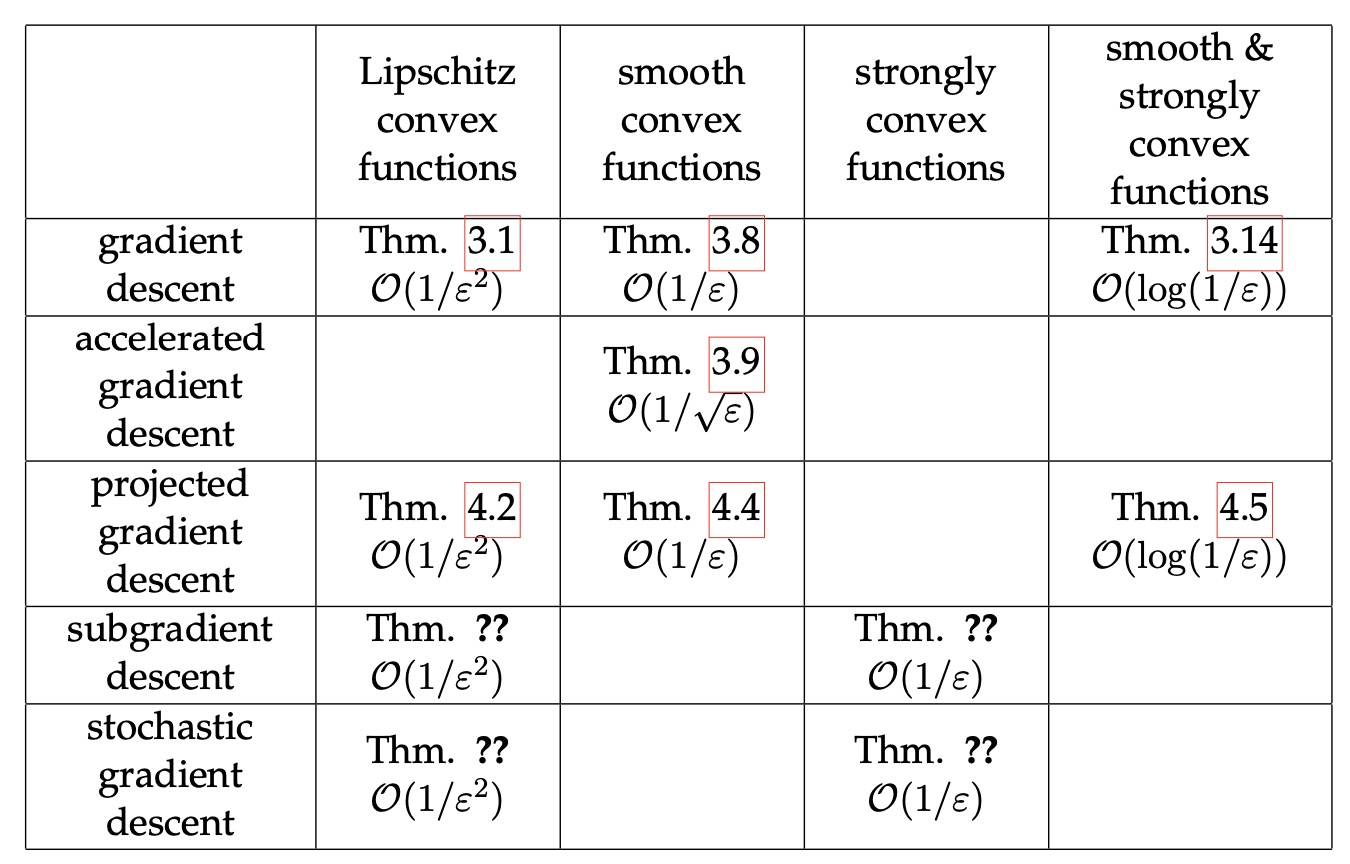
\includegraphics[width=\linewidth]{imgs/GD.jpg}

Define $g_t = \nabla f(x_t)$. The gradient descent is $x_{t+1} = x_t - \gamma g_t$, where $\gamma$ is the step size. We assume $f$ is differentiable anywhere.

\textbf{Definitions}:
\begin{enumerate}
    \item A convex differentiable function $f$ is $L$-smooth if $f(y) \le f(x) + \nabla f(x)^\top (y-x) + \frac{L}{2}\|x-y\|^2$ for any $x, y$.
    \item A function is $\mu$-strongly convex if $f(y) \ge f(x) + \nabla f(x)^\top (y-x) + \frac{\mu}{2}\|x-y\|^2$ for any $x, y$.
\end{enumerate}

\textbf{Properties}:
\begin{enumerate}
    \item \textbf{Characterization of $L$-smoothness (equivalent)}: (3.3) $\frac{L}{2}x^\top x - f(x)$ is convex; (3.5) $\|\nabla f(x) - \nabla f(y)\| \le L \|x-y\|$ for any $x,y$;
    \item \textbf{Operations that perserve smoothness} (3.6): (i) Assume $f_i$ are $L_i$-smooth and $\lambda_i >0$, then $f:= \sum_{i} \lambda_i f_i$ is $\sum_i \lambda_i L_i$-smooth. Proof by (3.3). (ii) Assume $f$ is $L$-smooth and $g(x) = Ax+b$, then $f\circ g$ is $L\|A\|^2$-smooth.
    \item \textbf{Characterization of $\mu$-strongly convexity (equivalent)}: (3.11) $f(x) - \frac{\mu}{2}x^\top x$ is convex.
    \item \textbf{Bound of first-order changes}: Let $f$ be convex and $x^*$ be the global minimum, i.e. $\nabla f(x^*) = 0$. If $f$ is $\mu$-strongly convex, then $\nabla f(x)^\top (x - x^*) \ge \mu \|x-x^*\|^2$. If $f$ is $L$-smooth, then $\nabla f(x)^\top (x - x^*) \le L \|x-x^*\|^2$. Proof: write definition separately for $x^*$ on $x_t$ and $x_t$ on $x^*$, then add the two inequalities together.
\end{enumerate}

Analysis based on the first-order characterization:
\begin{enumerate}
    \item Vanilla analysis (no further assumption): by first-order characterization, we can bound $f(x_t)-f(x^*) \le g_t^\top (x_t - x^*)$. The algorithm says $g_t = (x_t - x_{t+1}) / \gamma$, thus $g_t^\top (x_t - x^*) = \frac{1}{\gamma} (x_t - x_{t+1})^\top (x_t - x^*)$. Since $2a^\top b = a^\top a + b^\top b - (a-b)^\top (a-b)$, we have $2(x_t - x_{t+1})^\top (x_t - x^*) = \|x_t - x_{t+1}\|^2 + \|x_t - x^*\|^2 - \|x_{t+1} -x^*\|^2$. Therefore, $\sum_{t=0}^{T-1}(f(x_t)-f(x^*)) \le \sum_{t=0}^{T-1} g_t^\top (x_t - x^*) \le \frac{\gamma}{2}\sum_{t=0}^{T-1}\|g_t\|^2 + \frac{1}{2\gamma} \|x_0-x^*\|^2$.  The problem is to bound the squared norm of gradients.
    \item Lipschitz convex functions: bounded gradients $\|\nabla f(x)\| \le B$ for any $x$. (3.1) Assume $\|x_0 - x^*\| \le R$.  Then the result of vanilla analysis says $\sum_{t=0}^{T-1}(f(x_t)-f(x^*)) \le \frac{\gamma}{2}B^2 T + \frac{1}{2\gamma}R^2$. Choose $\gamma=\frac{R}{B\sqrt{T}}$ yields $\frac{1}{T}\sum_{t=0}^{T-1}(f(x_t)-f(x^*)) \le \frac{RB}{\sqrt{T}}$. This means we need $T\ge R^2B^2/\epsilon^2$ to achieve $\min_t (f(x_t)-f(x^*)) \le \epsilon$. 
\end{enumerate}

Analysis based on control over the quadratic term:
\begin{enumerate}
    \item $L$-smooth functions (not requiring convexity): (3.7) with $\gamma:=1/L$, we have $f(x_{t+1}) \le f(x_t) - \frac{1}{2L}\|\nabla f(x_t)\|^2$. Proof: use smoothness definition and plug in $x_{t+1}-x_t = -\frac{1}{L}\nabla f(x_t)$.
    \item Convex $L$-smooth functions: (3.8) with $\gamma:=1/L$, we have $f(x_T) - f(x^*) \le \frac{L}{2T}\|x_0 - x^*\|^2$. This means we only need $T \ge \frac{R^2 L}{2\epsilon}$ to achieve error at most $\epsilon$. Proof: by (3.7), $\frac{1}{2L}\sum_{t=0}^{T-1} \|\nabla f(x_t)\|^2 \le f(x_0) - f(x^*)$. Plugging into vanilla analysis, we have $\sum_{t=1}^T (f(x_t) - f(x^*)) \le \frac{L}{2}\|x_0 - x^*\|^2$. By (3.7), $f(x_t) - f(x^*)$ is monotonically decreasing, thus $f(x_T) - f(x^*) \le \frac{L}{2T}\|x_0 - x^*\|^2$. 
    \item $\mu$-strongly convex and $L$-smooth functions: (3.14) GD with $\gamma = 1/L$ yields $\|x_{t+1}-x^*\|^2 \le (1-\frac{\mu}{L})\|x_t - x^*\|^2$ and $f(x_T) - f(x^*) \le \frac{L}{2}(1-\frac{\mu}{L})^T \|x_0 -x^*\|^2$. This means we need $T \ge \frac{L}{\mu}\log\left(\frac{R^2 L}{2\epsilon}\right)$ to achieve error at most $\epsilon$. Proof: (i) replacing the first-order characterization in the vanilla analysis by the condition of $\mu$-strongly convexity, we get $\|x_{t+1}-x^*\|^2 \le 2\gamma \left(f(x^*) - f(x_t)\right) + \gamma^2 \|\nabla f(x_t)\|^2 + (1-\mu\gamma)\|x_t - x^*\|^2$. By sufficient decrease of $L$-smooth functions, we have $f(x^*) - f(x_t) \le f(x_{t+1}) - f(x_t) \le -\frac{1}{2L}\|\nabla f(x_t)\|^2$. Combining these two gives the first result. (ii) By smoothness, $f(x_T) - f(x^*) \le \frac{L}{2}\|x_T - x^*\|^2 \le \frac{L}{2}(1-\frac{\mu}{L})^T \|x_0 -x^*\|^2$. 
\end{enumerate}

\textbf{Optimizing without knowing $L$ or $B$}: for $L$-smooth convex functions, we do not need to know $L$ to ensure $O(\frac{R^2 L}{\epsilon})$ steps. The idea is to guess $L$ and refine it gradually. The first guess is $L_0 := \frac{2\epsilon}{R^2}$. For each guess, we check if the sufficient decrease (3.7) holds. If (3.7) holds in the whole process $T = \frac{R^2 L_i}{2\epsilon}$, then $L_i$ is a successful guess, and we finish. If the guess is incorrect, we double $L_{i+1} = 2L_i$ and repeat. The final guess cannot exceed two times the correct value, and the number of iterations is bounded by $\sum_i 2^i$ until the last term exceeds the true $L$. This means the total number of iterations is bounded by two times the last iteration time, which is still $O(\frac{R^2 L}{\epsilon})$. A similar approach can be taken for Lipschitz convex functions to optimize without knowing $B$.

\textbf{Accelerated Gradient Descent}

The AGD is to do $y_{t+1}= x_t - \frac{1}{L}\nabla f(x_t)$, $z_{t+1} = z_t - \frac{t+1}{2L}\nabla f(x_t)$ and $x_{t+1} = \frac{t+1}{t+3} y_{t+1} + \frac{2}{t+3}z_{t+1}$. Initialized with $y_0=z_0 = x_0$.

(Thm 3.9) For $L$-smooth convex functions, AGD yields $f(y_T) - f(x^*) \le \frac{2L\|z_0 - x^*\|^2}{T(T+1)}$.

\section{Projected Gradient Descent}

PGD: do constrainted gradient descent. $y_{t+1} = x_t - \gamma \nabla f(x_t)$ then $x_{t+1} = \Pi_X(y_{t+1}) = \argmin_{X} \|x - y_{t+1}\|^2$.

\textbf{projection inequalities} (4.1): let $X$ be closed and convex, $x\in X$, then $(x - \Pi_X(y))^\top (y - \Pi_X(y)) \le 0$ and $\|x - \Pi_X(y)\|^2 + \|y - \Pi_X(y)\|^2 \le \|x - y\|^2$. Proof: $\Pi_X(y)$ minimizes $f(x) = \|x- y\|^2$ on $Z$, thus by optimality, $\nabla f(\Pi_X(y))^\top (x - \Pi_X(y)) = 2(\Pi_X(y) - y)^\top (x - \Pi_X(y)) \ge 0$ for any $x \in X$. The second follows from $2a^\top b = \|a\|^2 + \|b\|^2 - \|a - b\|^2$. Illustration:
    \begin{center}
        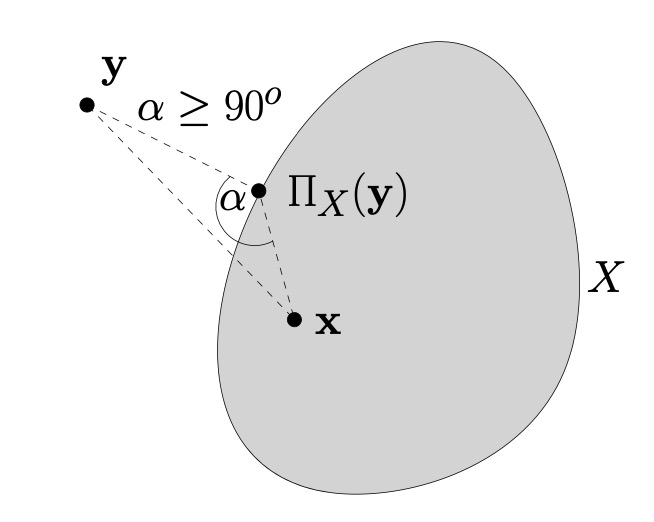
\includegraphics[width=.6\linewidth]{imgs/projection.jpg}
    \end{center}

\textbf{Analysis for PGD}: the same result but proof adapted using projection inequalities.
\begin{enumerate}
    \item Vanilla analysis: the same analysis for PGD gives $g_t^\top (x_t - x^*) = \frac{1}{2\gamma}\left(\gamma^2 \|g_t\|^2 + \|x_t - x^*\|^2 - \|y_{t+1}-x^*\|^2\right)$. By projection inequality, we have $\|x_{t+1} - x^*\|^2 \le \|y_{t+1} - x^*\|^2$. Thus, the result of vanilla analysis is the same.
    \item Lipschitz convex functions: (4.2) the same as GD since it only requires the result of vanilla analysis.
    \item $L$-smooth functions: (4.3) with $\gamma = 1/L$, we have $f(x_{t+1}) \le f(x_t) - \frac{1}{2L}\|\nabla f(x_t)\|^2 + \frac{L}{2}\|y_{t+1} - x_{t+1}\|^2$. In addition, $f(x_{t+1}) \le f(x_t)$. Proof: write the smoothness definition for $x_{t+1}$ for $x_t$. Replace $\nabla f(x_t)^\top (x_{t+1} - x_t)$ by $-L (y_{t+1} - x_t)^\top (x_{t+1} - x_t)$ and then apply $2a^\top b = \|a\|^2 + \|b\|^2 - \|a - b\|^2$ gives the first result. Since $\|y_{t+1} - x_{t+1}\| \le \|y_{t+1} - x_t\| = \gamma \|\nabla f(x_t)\|$, we have $f(x_{t+1}) \le f(x_t)$.
    \item Convex $L$-smooth functions: (4.4) the same result as GD. Proof: we use a tighter inequality for vanilla analysis. Instead of using $\|x_{t+1} - x^*\|^2 \le \|y_{t+1} - x^*\|^2$, we now use $\|x_{t+1} - x^*\|^2 + \|y_{t+1} - x_{t+1}\|^2 \le \|y_{t+1} - x^*\|^2$, so the vanilla analysis results in $\sum_{t=0}^{T-1} (f(x_t) - f(x^*)) \le \frac{1}{2L}\sum_{t=0}^{T-1} \|g_t\|^2 + \frac{L}{2}\|x_0 - x^*\|^2 - \frac{L}{2}\sum_{t=0}^{T-1} \|y_{t+1} - x_{t+1}\|^2$. Combining this with (4.3) gets the result.
    \item $\mu$-strongly convex and $L$-smooth functions: (4.5) PGD with $\gamma = 1/L$ yields $\|x_{t+1}-x^*\|^2 \le (1-\frac{\mu}{L})\|x_t - x^*\|^2$ and $f(x_T) - f(x^*) \le \frac{L}{2}(1-\frac{\mu}{L})^T \|x_0 -x^*\|^2 + (1-\frac{\mu}{L})^{T/2}\|\nabla f(x^*)\|\|x_0 - x^*\|$. This is still $O(\log(\frac{1}{\epsilon}))$ steps. Proof: $\mu$-strongly convexity strengthens the vanilla analysis to be $g_t^\top (x_t - x^*) \le \frac{1}{2\gamma}(\gamma^2 \|g_t\|^2 + \|x_t - x^*\|^2 - \|x_{t+1}-x^*\|^2 - \|y_{t+1} - x_{t+1}\|^2) - \frac{\mu}{2}\|x_t - x^*\|^2$. This makes the vanilla analysis to give $\|x_{t+1}-x^*\|^2 \le 2\gamma \left(f(x^*) - f(x_t)\right) + \gamma^2 \|\nabla f(x_t)\|^2 + (1-\mu\gamma)\|x_t - x^*\|^2 - \|y_{t+1} - x_{t+1}\|^2$. The extra $- \|y_{t+1} - x_{t+1}\|^2$ happens to compensate for the additional term from the $L$-smoothness, thus (i) follows. By smoothness, we have $f(x_T) - f(x^*) \le \|\nabla f(x^*)\| \|x_T - x^*\| + \frac{L}{2} \|x_T - x^*\|^2$, thus (ii) follows from (i).
\end{enumerate}

\textbf{Projecting into $L_1$ ball}: solve $\Pi_X(v) = \argmin_{\|x\|\le 1}\|x-v\|^2$. WLOG, assume $v_1 \ge v_2 \ge \dots v_d \ge 0$ and $\sum_i v_i > 1$. (4.11) We have $x_i^* = v_i - \theta_p$ for $i\le p$ and $x^*=0$ for $i>p$, where $\theta_p = \frac{1}{p}(\sum_{i=1}^p v_i -1)$ and $p=\max\{p \in [d]: v_p - \frac{1}{p}(\sum_{i=1}^p v_i - 1)>0\}$. This makes the projection $O(dlog d)$. Actually it can be improved to $O(d)$.

\section{PL Condition and Coordinate Descent}

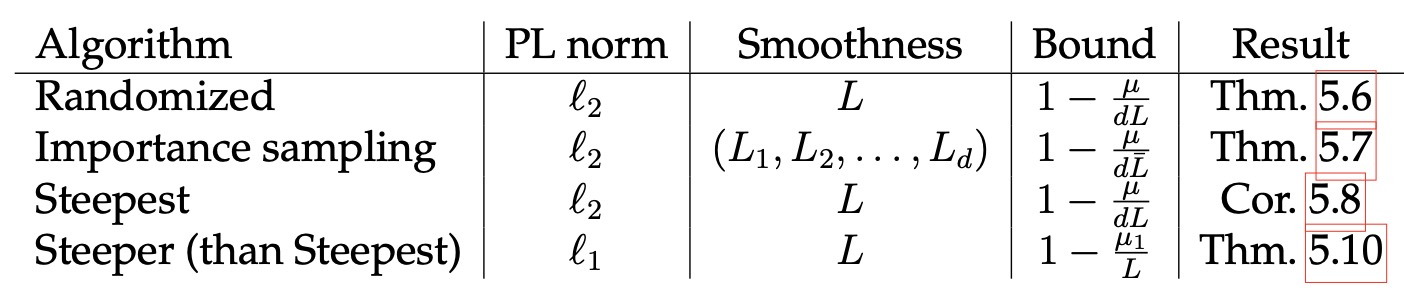
\includegraphics[width=\linewidth]{imgs/CGD.jpg}

\subsection{PL Condition}

\textbf{Definitions}:
\begin{enumerate}
    \item \textbf{Polyak-Lojasiewicz condition}: we say $f$ satisfies PL condition if $\frac{1}{2}\|\nabla f(x)\|^2 \ge \mu (f(x) - f(x^*))$.
    \item \textbf{Strong convexity w.r.t. $\|\cdot\|_1$}: $f(y) \ge f(x) + \nabla f(x)^\top (y-x) + \frac{\mu}{2}\|y-x\|_1^2$.
\end{enumerate}

\textbf{Properties}:
\begin{enumerate}
    \item \textbf{PL condition is weaker than strong convexity}: (5.2) if $f$ is $\mu$-strongly convex, then $f$ satisfies PL condition for the same $\mu$. Proof: by strong convexity, $f(x^*) - f(x) \ge \|\nabla f(x)\| \|y-x\| + \frac{\mu}{2} \|y-x\|^2 \ge -\frac{1}{2\mu}\|\nabla f(x)\|^2$.
    \item \textbf{PL condition is strictly weaker than strong convexity}: $f(x_1, x_2) = x_1^2$ is not strongly convex, but satisfies PL condition.
    \item \textbf{Smooth functions satisfying PL condition can be solved by GD in $O(\log(\frac{1}{\epsilon}))$}: for such functions, we have $f(x_T) - f(x^*) \le (1-\frac{\mu}{L})^T (f(x_0) - f(x^*))$. Proof: by sufficient descrease of $L$-smoothness, we have $f(x_{t+1}) \le f(x_t) - \frac{1}{2L}\|\nabla f(x_t)\|^2$. By PL condition, this means $f(x_{t+1}) \le f(x_t) - \frac{\mu}{L} (f(x_t) - f(x^*))$, which implies $f(x_{t+1}) - f(x^*) \le (1-\frac{\mu}{L}) (f(x_t) - f(x^*))$.
    \item \textbf{Strong convexity w.r.t. $\|\cdot\|_1$ and $\|\cdot\|_2$}: if $f$ is $\mu$-strongly convex w.r.t. $\|\cdot\|_1$, then $f$ is also $\mu$-strongly convex w.r.t. $\|\cdot\|_2$; if $f$ is $\mu$-strongly convex w.r.t. $\|\cdot\|_2$, then $f$ is $\mu / d$-strongly convex w.r.t. $\|\cdot\|_1$. Proof: use $\|x\|_1 \ge \|x\|_2$ and $\|x\|_2 \ge \frac{1}{\sqrt{d}}\|x\|_1$.
    \item \textbf{Strong convexity w.r.t. $\|\cdot\|_1$ implies PL condition w.r.t. $\|\cdot\|_\infty$}: (5.9) if $f$ has strong convexity w.r.t. $\|\cdot\|_1$, then $\frac{1}{2}\|\nabla f(x)\|_\infty^2 \ge \mu (f(x) - f(x^*))$. Proof: simply use $\nabla f(x)^\top (y-x) \le \|\nabla f(x)\|_\infty \|y-x\|_1$ in (5.2) instead.
\end{enumerate}


\subsection{Coordinate Descent}

\textbf{Coordinate-wise smoothness}: $f$ is called coordinate-wise smooth with parameter $L = (L_1, \dots, L_d)$ if for every coordinate $i$ we have $f(x + \lambda e_i) \le f(x) + \lambda \nabla_i f(x) + \frac{L_i}{2} \lambda^2$.

\textbf{Coordinate Descent Algorithm}: for each iteration $t$, choose an active coordinate $i \in [d]$, then do $x_{t+1} = x_t - \gamma_i \nabla_i f(x_i) e_i$.

\textbf{Sufficient decrease}: (5.5) with $\gamma_i = 1 / L_i$, we have $f(x_{i+1}) \le f(x_i) - \frac{1}{2L_i} |\nabla_i f(x_t)|^2$. Proof: plugging the update step into the definition of coordinate-wise smoothness immediately gives the result.

\textbf{Analysis for coordinate-wise smooth functions satisfying PL condition}:
\begin{enumerate}
    \item \textbf{Randomized coordinate descent}: (5.6) choose coordinate uniformly at random and set $\gamma_i = 1/L$ where $L = \max_i L_i$, the randomized coordinate descent gets $\E(f(x_T) - f(x^*)) \le (1-\frac{\mu}{d L})^T (f(x_0) - f(x^*))$. This means randomized coordinate descent is the same good as GD, as the number of iterations is $d$ times higher, but each iteration is $d$ times cheaper. Proof: by sufficient decrease of coordinate descent, $\E (f(x_{t+1}) \mid x_t) \le f(x_t) - \frac{1}{2L} \sum_{i=1}^d \frac{1}{d} |\nabla_i f(x_t)|^2 = f(x_t) - \frac{1}{2dL} \|\nabla f(x_t)\|^2$. By PL condition, this means $\E (f(x_{t+1}) \mid x_t) \le f(x_t) - \frac{\mu}{dL}(f(x_t) - f(x^*))$, which implies $\E(f(x_{t+1}) - f(x^*) \mid x_t) \le (1-\frac{\mu}{dL})(f(x_t) - f(x^*))$. This means $\E(f(x_{t+1}) - f(x^*)) \le (1-\frac{\mu}{dL})\E(f(x_t) - f(x^*))$.
    \item \textbf{Importance sampling}: (5.7) choose coordinate $i$ with probability $\frac{L_i}{\sum_j L_j}$ and define $\bar{L} = \frac{1}{d}\sum_{i=1}^d L_i$, we have $\E(f(x_T) - f(x^*)) \le (1-\frac{\mu}{d\bar{L}})^T (f(x_0) - f(x^*))$. Note how randomized coordinate descent for $L$-smooth functions is a special case of this result. Proof: $\E (f(x_{t+1}) \mid x_t) \le f(x_t) - \frac{1}{2} \sum_{i=1}^d \frac{L_i}{\sum_j L_j} \frac{1}{L_i} |\nabla_i f(x_t)|^2 = f(x_t) - \frac{1}{2d\bar{L}}\sum_i |\nabla_i f(x_t)|^2$. The rest is the same to (5.6).
    \item \textbf{Steepest coordinate descent}: (5.8) choose coordinate $i = \argmax_i |\nabla_i f(x_t)|$, we have $f(x_T) - f(x^*) \le (1-\frac{\mu}{d L})^T (f(x_0) - f(x^*))$. Proof: simply remove the expectation and use maximum is greater than average.
    \item \textbf{Steepest descent for strong convexity w.r.t. $\|\cdot\|_1$}: (5.10) if $f$ is $\mu_1$-strongly convex w.r.t. $\|\cdot\|_1$, then with $\gamma_i = 1/L$, steepest descent gives $f(x_T) - f(x^*) \le (1- \frac{\mu_1}{L})^T (f(x_0) - f(x^*))$. Note that steepest descent has the same per iteration cost as GD, but the $\mu_1$ could be greater than the $L_2$ strong convexity parameter. Proof: by sufficient decrease and the update rule, $f(x_{t+1}) \le f(x_t) - \frac{1}{2L}\|\nabla f(x_t)\|_\infty^2$. By the PL condition w.r.t. $\|\cdot\|_\infty$, this means $f(x_{t+1}) \le f(x_t) - \frac{\mu_1}{L} (f(x_t) - f(x^*))$ and thus $f(x_{t+1}) - f(x^*) \le (1- \frac{\mu_1}{L})(f(x_t) - f(x^*))$.
    \item \textbf{Greedy coordinate descent}: choose some coordinate, then do $x_{t+1} = \argmin_\lambda f(x_t + \lambda e_i)$, i.e., make the largest step possible. For differentiable convex functions, as the update can only be better than before, it does not compromise the analysis. For non-differentiable case, however, it may get stuck in non-optimal points. (5.11) Assume $f(x) = g(x) + h(x)$, where $h(x) = \sum_i h_i (x_i)$, $g$ is convex and differentiable and $h_i$ is convex, then if the greedy descent converges, it converges to the global minimum of $f$. Such $h$ is called \emph{separable}, which includes $L_1$ norm and squared $L_2$ norm. This means LASSO and ridge objectives are concrete cases. Proof: $f$ is the sum of convex functions, thus convex. Let $x$ be the converged point and $y$ be a near point. Thus, $\nabla_i g(x) (y_i - x_i) + h_i(y_i) - h_i(x_i) \ge 0$, since the algorithm converges. By first-order characterization, we have $f(y) - f(x) \ge \nabla g(x)^\top (y-x) + \sum_i (h_i(y_i) - h_i(x_i)) \ge 0$.
\end{enumerate}

\section{Subgradient Methods}

\textbf{Separating plane of two convex sets}: let $S$ and $T$ be two nonempty convex sets. A hyperplane $a^\top x = b$ is said to separate $S$ and $T$ if $S \cup T \not\subset H$, $S \subset H^-=\{x: a^\top x \le b\}$ and $T \subset H^+ = \{x: a^\top x \ge b\}$. If further $S \subset H^{--}=\{x: a^\top x < b\}$ and $T \subset H^{++} = \{x: a^\top x > b\}$, then $H$ is said to strictly separate $S$ and $T$.

\textbf{Hyperplane separation theorem}: for two non-empty convex sets $S$ and $T$, they can be separated by a hyperplane iff $\rint(S) \cap \rint(T) = \emptyset$.

\textbf{Definitions}:
\begin{enumerate}
    \item \textbf{Subgradient}: let $f$ be a convex function, then a vector $g$ is a subgradient of $f$ at $x$ if $f(y) \ge f(x) + g^\top (y-x)$.
    \item \textbf{Subdifferential}: the set of all subgradient at $x$ is called the subdifferential of $f$ at $x$, denoted as $\partial f$.
    \item \textbf{Directional derivative}: the directional derivative of $f$ at $x$ along $d$ is $f^\prime(x;d) = \lim_{\delta \rightarrow 0^+} \frac{f(x+\delta d) - f(x)}{\delta}$.
\end{enumerate}

\textbf{Properties}:
\begin{enumerate}
    \item \textbf{subgradient = gradient, when convex and differentiable}: (6.2) if $f$ is convex and differentiable at $x$, then $\partial f=\{\nabla f(x)\}$; (6.3) if $f$ is only differentiable but not convex, then $\partial f \subseteq \{\nabla f(x)\}$. Proof: clearly $\{\nabla f(x)\} \subseteq \partial f$ given $f$ convex; assume $\partial f \ne \emptyset$, let $y = x+\epsilon d$ for small $\epsilon$, then $\frac{f(y) - f(x)}{\epsilon} \ge g^\top d$, which means $\nabla f(x)^\top d \ge g^\top d$ for any $d$. This implies $g = \nabla f(x)$.
    \item \textbf{Bounded subgradient for convex functions = Lipschitz}: (6.5) if $f$ is convex and $\dom(f)$ is open, then $\|g\| \le B$ for all $x$ and $g \in \partial f(x)$ is equivalent to $|f(x)-f(y)| \le B \|x-y\|$ for all $x,y$. Proof: (i) one side: let $y=x+\epsilon g$ for some $\epsilon >0$. Then $f(y)-f(x) \ge \epsilon \|g\|^2$. By $B$-Lipschitz, $f(y) -f(x) \le B\|y-x\| = \epsilon B \|g\|$. These two imply $\|g\|\le B$. (ii) the other side: for any $x,y$ and $g \in \partial f(x)$, $f(x) - f(y) \le g^\top (x-y) \le \|g\|\|x-y\| \le B\|x-y\|$ and $f(y) - f(x) \ge g^\top (y-x) \ge -B \|y-x\|$.
    \item \textbf{Convexity means subgradient almost everywhere}: (6.10) let $f$ be convex and $x \in \rint(\dom(f))$, then $\partial f(x)$ is non-empty and bounded. Proof: (i) non-emptiness: w.l.o.g, assume $\dom(f)$ is full-dimensional and $x \in \text{int}(\dom(f))$. Since $\epi(f)$ is convex, by hyperplane separation theorem, $\exists s, \beta$, s.t. $s^\top y + \beta t \ge s^\top x + \beta f(x)$ for any $(y,t) \in \epi(f)$. Since $t$ can be arbitratily large, we have $\beta \ge 0$. If $\beta = 0$, then $s^\top (y-x) \ge 0$ for any $y$, which means $s=0$, a contradiction. Thus, $\beta > 0$. Setting $g = -\beta^{-1} s$, we get $f(y) \ge f(x) + g^\top (y-x)$. (ii) boundness: suppose $\exists g_k \in \partial f(x)$ s.t. $\|g_k\| \rightarrow +\infty$. Since $x\in\text{int}(\dom(f))$, $\exists \delta>0$, s.t. $B(x, \delta) \subseteq \dom(f)$. Therefore, $y_k := x+\delta \frac{g_k}{\|g_k\|} \in \dom(f)$. By definition, $f(y_k) \ge f(x) + g_k^\top (y_k - x) = f(x) + \delta \|g_k\| \rightarrow +\infty$, a contradition.
    \item \textbf{Subgradient everywhere means convexity}: if $\dom(f)$ is convex and for any $x \in \dom(f)$, $\partial f(x)$ is non-empty, then $f$ is convex. Proof: for any $x, y \in \dom(f)$ and $\lambda \in (0,1)$, let $z = \lambda x + (1-\lambda) y$ and $g \in \partial f(z)$. Then $f(x) \ge f(z) + g^\top (x-z)$ and $f(y) \ge f(z) + g^\top (y-z)$. Adding them leads to definition of convexity.
    \item \textbf{$\text{dist}(0, \partial f(x))$ decides optimality}: if $0 \in \partial f(x)$, then $x$ is a global minimum. Proof: by definition.
    \item \textbf{Subgradient and directional derivative}: (6.13) let $f$ be convex and $x \in \text{int}(\dom(f)),$ then $f^\prime(x ;d) = \max_{g \in \partial f(x)} g^\top d$. Proof: by the definition of subgradient. we have $f(x+\delta d) - f(x) \ge \delta g^\top d$, which implies $f^\prime(x ; d) \ge g^\top d$ for any $g \in \partial f(x)$ and thus $f^\prime(x ; d) \ge \max_{g \in \partial f(x)} g^\top d$. To conclude the other side, consider $C_1 = \{(y,t): f(y)<t\}$ and $C_2 = \{(y,t): y=x+\alpha d, t = f(x)+\alpha f^\prime(x;d), \alpha \ge 0\}$. Clearly they are convex and non-empty. If $C_1 \cap C_2 = \emptyset$, then by hyperplane separation theorem, $\exists g_0, \beta$, s.t. $g_0^\top (x+\alpha d) + \beta (f(x) + \alpha f^\prime(x;d)) \le g_0^\top y + \beta t$ for any $\alpha \ge 0$ and any $t > f(y)$. Similar to the proof of (6.10), we can show $\beta > 0$. Let $\tilde{g}=\beta^{-1} g_0$, we have $\tilde{g}^\top (x+\alpha d) + f(x) + \alpha f^\prime(x;d) \le \tilde{g}^\top y + f(y)$ . Set $\alpha = 0$, we have $\tilde{g}x + f(x) \le \tilde{g}^\top y + f(y)$, which means $-\tilde{g} \in \partial f(x)$. Further, set $y=x$ and $\alpha=1$, we have $f^\prime(x;d) \le - \tilde{g}^\top d \le \max_{g \in \partial f(x)} g^\top d$.
\end{enumerate}

\textbf{Calculus of subgradient}:
\begin{enumerate}
    \item For $h(x) = \lambda f(x) + \mu g(x)$ where $\lambda, \mu \ge 0$ and $f,g$ both are convex, then $\partial h(x) = \lambda \partial f(x) + \mu \partial g(x)$.
    \item For $h(x) = f(Ax+b)$ where $f$ is convex, then $\partial h(x) = A^\top \partial f(Ax+b)$.
    \item For $h(x) = \sup_{\alpha \in A} f_\alpha(x)$ and each $f_\alpha(x)$ is convex, then $\partial h(x) \supseteq \text{conv}\{\partial f_\alpha(x): f_\alpha(x) = h(x)\}$.
    \item For $h(x) = F(f_1(x), \dots, f_m(x))$ where $F$ is non-decreasing and convex, then $\partial h(x) \supseteq \{\sum_{i=1}^m d_i \partial f_i(x): (d_1, \dots, d_m) \in \partial F(y_1, \dots, y_m)\}$.
\end{enumerate}

\subsection{Subgradient descent} 
Consider $f$ convex (possibly non-differentiable) on a closed and convex set $X$. The subgradient descent does $x_{t+1} = \Pi_X(x_t - \gamma_t g(x_t))$, where $g(x_t) \in \partial f(x_t)$. When $f$ is differentiable, this reduces to PGD. However, moving towards the negative direction of subgradient is not necessarily decreasing the objective. Therefore, we can only measure $\min_{t \le T} f(x_t) - f^*$ instead of $f(x_T)-f^*$.

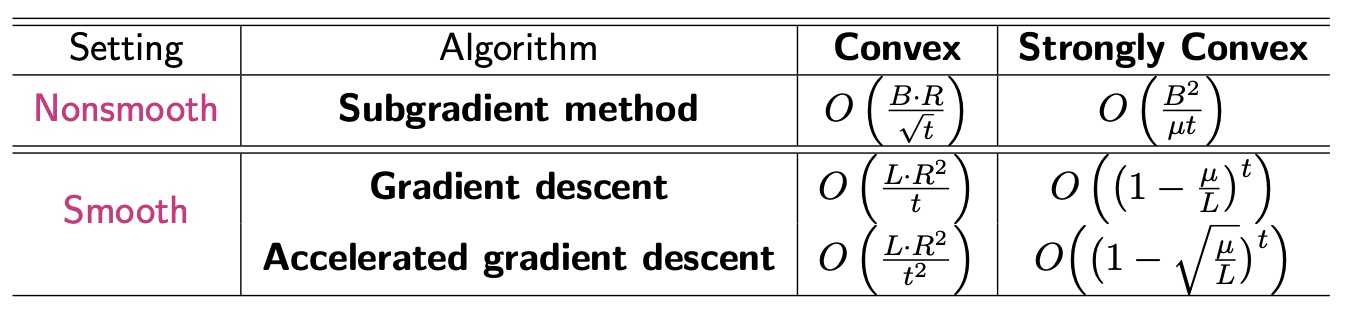
\includegraphics[width=\linewidth]{imgs/subGD.jpg}

\textbf{Analysis for convex functions}:
\begin{enumerate}
    \item \textbf{General analysis}: (6.17) starting from $x_1$, we have $\min_{1\le t\le T} f(x_t) - f^* \le \frac{1}{2}(\sum_{t=1}^T \gamma_t)^{-1}(\|x_1 - x^*\|^2 + \sum_{t=1}^T \gamma_t^2\|g(x_t)\|^2)$ and $f(\hat{x}_T) - f^* \le \frac{1}{2}(\sum_{t=1}^T \gamma_t)^{-1}(\|x_1 - x^*\|^2 + \sum_{t=1}^T \gamma_t^2\|g(x_t)\|^2)$ for $\hat{x}_t=(\sum_{t=1}^T \gamma_t)^{-1}(\sum_{t=1}^T \gamma_t x_t)$. Proof: by definition, $\|x_{t+1} - x^*\|^2 = \|\Pi_X(x_t - \gamma_t g(x_t)) - x^*\|^2 \le \|x_t - \gamma_t g(x_t) - x^*\|^2 = \|x_t - x^*\|^2 - 2\gamma_t g(x_t)^\top (x_t - x^*) + \gamma_t^2\|g(x_t)\|^2$. By definition of subgradient, we have $f(x_t) - f^* \le g^\top (x_t - x^*)$. These two gives $\sum_{t=1}^T \gamma_t (f(x_t) - f^*) \le \frac{1}{2}(\|x_1 - x^*\|^2 - \|x_{T+1} - x^*\|^2 + \sum_{t=1}^T \gamma_t^2\|g(x_t)\|^2) \le \frac{1}{2}(\|x_1 - x^*\|^2 + \sum_{t=1}^T \gamma_t^2\|g(x_t)\|^2)$. In addition, we have $\min_{t} f(x_t) - f^* \le (\sum_{t=1}^T \gamma_t)^{-1} (\sum_t \gamma_t (f(x_t) - f^*))$, thus the first claim follows. For the second claim, use $\sum_t \gamma_t (f(x_t) - f^*) \ge (\sum_t \gamma_t) (f(\hat{x}_t) - f^*)$ by convexity.
    \item \textbf{Lipschitz functions}: assume $\|x_1 - x^*\| \le R$ and $\|g(x_t)\| \le B$, then $\min f(x_t) - f^* \le \frac{1}{2}(\sum_{t=1}^T \gamma_t)^{-1} (R^2 + \sum_t \gamma_t^2 B^2)$.
\end{enumerate}

\textbf{$O(1/\sqrt{t})$ convergence under different stepsizes for  convex Lipschitz functions}:
\begin{enumerate}
    \item $\gamma_t = \gamma$: $\epsilon_t = \frac{1}{2}(\frac{R^2}{T\gamma} + B^2\gamma) \rightarrow \frac{B^2}{2}\gamma$. Choose $\gamma_t = \frac{R}{B\sqrt{T}}$, we have $\epsilon_t \le \frac{RB}{\sqrt{T}}$.
    \item $\sum_t \gamma_t \rightarrow +\infty$ and $\gamma_t \rightarrow 0$: we have $\epsilon_t \rightarrow 0$. If set $\gamma_t = \frac{R}{B\sqrt{t}}$, we get $\epsilon_t = O(\frac{BR}{\sqrt{T}})$
    \item $\sum_t \gamma_t \rightarrow +\infty$ and $\sum_t \gamma_t^2 < +\infty$: $\epsilon_t \rightarrow 0$.
    \item Polyak stepsize $\gamma_t = \frac{f(x_t) - f^*}{\|g(x_t)\|^2}$: this makes the general analysis to give $\|x_{t+1} - x^*\|^2 \le \|x_t - x^*\|^2 - 2\gamma_t g(x_t)^\top (x_t - x^*) + \gamma_t^2 \|g(x_t)\|^2 \le \|x_t - x^*\|^2 - 2\gamma_t (f(x_t) - f^*) + \gamma_t^2 \|g(x_t)\|^2 = \|x_t - x^*\|^2 - \frac{(f(x_t) - f^*)^2}{\|g(x_t)\|^2} \le  \|x_t - x^*\|^2 - \frac{(f(x_t) - f^*)^2}{B^2}$, thus guarantees the decrease of $\|x_t - x^*\|$. This implies $\sum_t (f(x_t) - f^*)^2 \le R^2 B^2$, thus $\epsilon_t = O(\frac{RB}{\sqrt{T}})$.
\end{enumerate}

\textbf{$O(1/t)$ convergence for strongly convex Lipschitz functions}:
\begin{enumerate}
    \item (6.18) Let $f$ be $\mu$-strongly convex. With $\gamma_t = \frac{1}{\mu t}$, we have $\min f(x_t) - f^* \le \frac{B^2(\log(T)+1)}{2\mu T}$ and $f(\hat{x}_T) - f^* \le \frac{B^2(\log(T)+1)}{2\mu T}$ for $\hat{x}_T = \frac{1}{T}\sum_t x_t$. Proof: by strong convexity, $f(y) - f(x) + g(x)^\top (y-x) + \frac{\mu}{2}\|y-x\|^2$. Thus, general analysis gives $\|x_{t+1} - x^*\|^2 \le \|x_t-x^*\|^2 - 2\gamma_t (f(x_t) - f^* + \frac{\mu}{2}\|x_t - x^*\|^2) + \gamma_t^2 \|g(x_t)\|^2$, which implies an upper bound on $f(x_t) - f^*$. Following the same steps in the general analysis, we get the desired result.
    \item (6.19) Let $f$ be $\mu$-strongly convex. With $\gamma_t = \frac{2}{\mu (t+1)}$, we have $\min f(x_t) - f^* \le \frac{2B^2}{\mu (T+1)}$ and $f(\hat{x}_T) - f^* \le \frac{2B^2}{\mu (T+1)}$ for $\hat{x}_T = \sum_t \frac{2t}{T(T+1)} x_t$. Proof: the same analysis gives $t(f(x_t) - f^*) \le \frac{\mu t(t-1)}{4}\|x_t - x^*\|^2 - \frac{\mu t (t+1)}{4}\|x_{t+1}-x^*\|^2 + \frac{B^2}{\mu (t+1)}$. The result follows.
\end{enumerate}

\textbf{Subgradient descent is asymptotically optimal for first-order subgradient methods}: (Thm 6.20): for any $1\le t \le n$ and $x_1 \in \mathbb{R}^n$, there exists a $B$-Lipschitz continuous function $f$ and a convex set $X$ with diameter $R$, s.t. for any first-order method that generates $x_t \in x_1 + \text{span}(g(x_1), \dots, g(x_{t-1}))$, where $g(x_i) \in \partial f(x_i)$, we have $\min_{1\le s\le t}f(x_s) - f^* \ge \frac{BR}{4(1+\sqrt{t})}$. In addition, there exists a $B$-Lipschitz continuous function $f$ that is $\mu$-strongly convex, s.t. $\min_{1\le s\le t}f(x_s) - f^* \ge \frac{B^2}{8\mu t}$. Proof: W.l.o.g., assume $x_1=0$. Let $X = \{x:\|x\| \le R/2\}$ and $f(x) =  C\max_{1\le i\le t}x_i + \frac{\mu}{2}\|x\|^2$ for some $C>0, \mu >0$. The subgradient of $f$ is $\partial f(x) = \mu x + C \cdot \text{conv}\{e_i: i \text{ s.t. } x_i=\max_{1\le j \le t}x_j\}$. The optima of $f$ is $f^* = - \frac{C^2}{2\mu t}$. Consider $g(x)=Ce_i+\mu x$, where $i$ is the first coordinate that $x_i = \max_{1\le j \le t} x_j$. Since the algorithm runs for $t$ iterations, the last dimension cannot be updated. Therefore, $\min_{1\le s \le t}f(x_s) - f^* \ge \frac{C^2}{2\mu t}$. (1) Let $C = \frac{B\sqrt{t}}{1+\sqrt{t}}$ and $\mu = \frac{2B}{R(1+\sqrt{t})}$, we have $\max_{g \in \partial f(x)}\|g\| \le C + \mu \|x\|\le R$, and the first result follows. (2) Let $C=\frac{B}{2}$ and $\mu = \frac{B}{R}$, we have $\max_{g \in \partial f(x)}\|g\| \le C + \mu \|x\|\le R$, $f$ is $\mu$-strongly convex, and the second result follows.

\subsection{Mirror Descent}

Mirror descent only uses subgradients, and have the same aymptotic performance as subgradient descent. However, it may have better constants than subgradient descent. Subgradient descent is a special case of mirror descent.

\textbf{Definitions}:
\begin{enumerate}
    \item \textbf{Bregman Divergence}: let $w(x)$ be strictly convex and continuously differentiable on a close convex $X$. $V_w(x, y) = w(x) - w(y) - \nabla w(y)^T (x-y)$ is defined to be the Bregman divergence. This is asymmetric, thus not a valid distance. If $w$ is $\mu$-strongly convex, then $V_w(x, y)$ is $\mu$-strongly convex in $x$.
    \item \textbf{Prox-mapping}: given an input $x$ and vector $\xi$, the prox-mapping is defined as $\Prox_x(\xi) = \argmin_{u\in X}\{V_w(u, x) + \langle \xi, u \rangle\}$, where $w$ is $1$-strongly convex. 
    \item \textbf{Mirror Descent}: do $x_{t+1} = \Prox_{x_t}(\gamma_t g(x_t)) = \argmin_{x\in X}\{w(x)+\langle \gamma_t g(x_t)-\nabla w(x_t), x\rangle\}$. Recall that the subgradient descent is equivalent to $x_{t+1}=\argmin_{x \in X} \{\frac{1}{2}\|x-x_t\|^2 + \langle \gamma_t g(x_t), x\rangle\}$ and $V_w(x,y)=\frac{1}{2}\|x-y\|^2$ for $w(x) = \frac{1}{2}\|x\|^2$. Therefore, subgradient descent is a special case of mirror descent.
\end{enumerate}

\textbf{Properties}:
\begin{enumerate}
    \item \textbf{Three point identity}: (6.26) $V_w(x, z) = V_w(x, y) + V_w(y, z) - \langle \nabla w(z) - \nabla w(y), x-y \rangle$. Proof: by definition.
    \item \textbf{Generalized Pythagorean Theorem for Bregman Divergence}: (6.23) if $x^* = \argmin_{x \in C} V_w(x, x_0)$ for some convex set $C$, then for any $y \in C$, we have $V_w(y, x_0) \ge V_w(y, x^*) + V_w(x^*, x_0)$. Proof: use $\nabla V_w(x, x_0)^\top \mid_{x=x^*} (y-x^*) \ge 0 \Leftrightarrow (\nabla w(x^*) - \nabla w(x_0))^\top (y-x^*) \ge 0$ and the three point identity.
    \item \textbf{Convergence of mirror descent}: (6.28) let $f$ be convex, we have $\min_{1 \le t \le T}f(x_t) - f^* \le \frac{1}{\sum_{t=1}^T \gamma_t} (V_w(x^*, x_1) + \frac{1}{2}\sum_{t=1}^T \gamma_t^2 \|g(x_t)\|^2)$. Proof: since $x_{t+1} =  \argmin_{x\in X}\{w(x)+\langle \gamma_t g(x_t)-\nabla w(x_t), x\rangle\}$, by optimality we have $\langle \nabla w(x_{t+1}) + \gamma_t g(x_t) - \nabla w(x_t), x-x_{t+1}\rangle \ge 0$. Therefore, we have $\langle \gamma_t g(x_t), x_{t+1} -x \rangle \le \langle \nabla w(x_{t+1}) - \nabla w(x_t), x-x_{t+1} \rangle = V_w(x, x_t) - V_w(x, x_{t+1}) - V_w(x_{t+1}, x_t)$. Using $\langle \gamma_t g(x_t), x_t - x_{t+1}\rangle \le \frac{\gamma_t^2}{2}\|g(x_t)\|^2 + \frac{1}{2}\|x_t - x_{t+1}\|^2$ and noticing $V_w(x_{t+1}, x_t) \ge \frac{1}{2}\|x_t - x_{t+1}\|^2$ by 1-strongly convexity, we have $\langle \gamma_t g(x_t), x_t - x^* \rangle \le V_w(x^*, x_t) - V_w(x^*, x_{t+1}) + \frac{\gamma_t^2}{2}\|g(x_t)\|^2$. The rest is the same as the proof of (6.17).
\end{enumerate}


\section{Stochastic Optimization}

The goal is to $\min_{x \in X} F(x) = \frac{1}{n}\sum_{i=1}^n f_i(x)$, or more generally, $\min_{x \in X} F(x) = \E_\xi (f(x, \xi))$. For large $n$, computing the full gradient is expensive. For unknown $P(\xi)$, the gradient is intractable.

\textbf{Stochastic gradient quality for smooth functions}: (12.12) let $F(x)=\frac{1}{n}\sum_{i=1}^n f_i(x)$, where $f_i$ is $L_i$-smooth and convex, and $F$ has a global minimum $x^*$. Let $L_{\text{max}} = \max_i\{L_i\}$, then for any $x$ we have $\frac{1}{n}\sum_{i=1}^n \|\nabla f_i(x) - \nabla f_i(x^*)\|^2 \le 2L_{\text{max}}(F(x) - F(x^*))$. Proof: define $g_i(x) = f_i(x) - f_i(x^*) - \nabla f_i(x^*)^\top (x-x^*)$. Thus, $g_i(x)\ge 0$, and is convex and $L_i$-smooth. By sufficient decrease, we have $0\le g_i(x - \frac{1}{L_i}\nabla g_i(x)) \le g_i(x) - \frac{1}{2L_i}\|\nabla g_i(x)\|^2$. Thus, $g_i(x) \ge \frac{1}{2L_{\text{max}}}\|\nabla g_i(x)\|^2$. Expanding this by definition, summing over $i$, and using $\nabla F(x^*)=0$ yields the result. Note that the proof works for the general $F(x) = \E(x,\xi)$.

\textbf{Stochastic gradient descent}: do $x_{t+1} = \Pi_X (x_t - \gamma_t \nabla f(x_t, \xi_t))$. In the finite-sum problem, this is $x_{t+1} = \Pi_X(x_t - \gamma_t \nabla f_{i_t}(x_t))$, where $i_t$ is sampled uniformly at random. Thus, the \emph{gradient is unbiased}: $\E_{i_t} (\nabla f_{i_t} (x_t) \mid x_t) = \sum_i \frac{1}{n} \nabla f_i (x_t) = \nabla F(x_t)$, or $\E(\nabla f(x_t, \xi_t) \mid \xi_{[t-1]}) = \nabla F(x_t)$. The step size should diminish, i.e., $\gamma_t \rightarrow 0$, to ensure convergence, as the stochastic gradient does not necessarily equal to zero at the optima.

\textbf{Analysis}:
\begin{enumerate}
    \item \textbf{Strongly convex functions}: (12.3) assume $F(x)$ is $\mu$-strongly convex and $\E(\|\nabla f(x, \xi)\|^2) \le B^2$ for any $x \in X$. With $\gamma_t = \gamma / t$ for $\gamma > \frac{1}{2\mu}$, SGD satisfies $\E(\|x_t - x^*\|^2) \le \frac{C(\gamma)}{t}$, where $C(\gamma) = \max \{\frac{\gamma^2 B^2}{2\mu\gamma -1}, \|x_1 - x^*\|^2\}$. Proof: by projection inequality, $\|x_{t+1} - x^*\|^2 \le \|x_t - \gamma_t \nabla f(x_t, \xi_t) - x^*\|^2 = \|x_t - x^*\|^2 - 2\gamma_t \langle \nabla f(x_t, \xi_t), x_t - x^* \rangle + \gamma_t^2 \|\nabla f(x_t, \xi_t)\|^2$. Taking expectation, we have $\E(\|x_{t+1} - x^*\|^2) \le \E(\|x_t - x^*\|^2) - 2\gamma_t \E(\langle \nabla f(x_t, \xi_t), x_t - x^*\rangle) + \gamma_t^2 B^2$. Note that  $\E(\langle \nabla f(x_t, \xi_t), x_t - x^*\rangle) = \E\left[\E(\langle\nabla f(x_t, \xi_t), x_t-x^*\rangle \mid \xi_{[t-1]})\right] = \E(\langle \nabla F(x_t), x_t - x^*\rangle)$. By strong convexity, $\langle \nabla F(x_t), x_t - x^* \rangle \ge \mu \|x_t - x^*\|^2$, thus $\E(\|x_{t+1} - x^*\|^2) \le (1-2\mu \gamma_t)\E(\|x_t - x^*\|^2) + \gamma_t^2 B^2$. The result follows by induction.
    \item \textbf{Convex functions}: (12.4) let $F$ be convex and $\E(\|\nabla f(x, \xi)\|^2) \le B^2$ for any $x \in X$. SGD satisfies $\E(F(\hat{x_T}) - F(x^*)) \le \frac{R^2 + B^2 \sum_{t=1}^T \gamma_t^2}{2\sum_{t=1}^T \gamma_t}$ for $\hat{x_T} = \frac{\sum_{t=1}^T \gamma_t x_t}{\sum_{t=1}^T \gamma_t}$. Proof: use $\langle \nabla F(x_t), x_t - x^* \rangle \ge F(x_t) - F(x^*)$ in the proof of (12.3) gives $\gamma_t \E(F(x_t) - F(x^*)) \le \frac{1}{2}\E(\|x_t -x^*\|^2) - \frac{1}{2}\E(\|x_{t+1} - x^*\|^2) + \frac{1}{2}\gamma_t^2 B^2$. The result follows by recursion and convexity.
    \item \textbf{Strongly convex and smooth functions, constant step size}: (12.5) assume $F(x)$ is both $\mu$-strongly convex and $L$-smooth, and $\E(\|\nabla f(x, \xi)\|^2) \le \sigma^2 + c\|\nabla F(x)\|^2$. Then, with $\gamma_t = \gamma \le \frac{1}{Lc}$, $\E(F(x_t) - F(x^*)) \le \frac{\gamma L \sigma^2}{2\mu} + (1-\gamma \mu)^{t-1}(F(x_1) - F(x^*))$.
    \item \textbf{Non-convex but smooth function}: (12.8) assume $F(x) = \E(f(x, \xi))$ is $L$-smooth and $\E(\|\nabla f(x, \xi) - \nabla F(x)\|^2) \le \sigma^2$, then with $\gamma_t = \min\{1/L, \frac{\gamma}{\sigma\sqrt{T}}\}$, SGD achieves $\E(\|\nabla F(\hat{x}_T)\|^2) \le \frac{\sigma}{T}\left(2(F(x_1) - F(x^*))/\gamma + L\gamma\right)$, where $\hat{x}_T$ is selected uniformly at random from $\{x_1, \dots, x_T\}$. Proof: by $L$-smoothness and $x_{t+1}=x_t-\gamma_t \nabla f(x_t, \xi_t)$, we have $\E(F(x_{t+1}) - F(x_t)) \le \E(\nabla F(x_t)^\top (x_{t+1} - x_t) + \frac{L}{2}\|x_{t+1} - x_t\|^2) \le \E(-\gamma_t \nabla F(x_t)^\top \nabla f(x_t, \xi_t) + \frac{L\gamma_t^2}{2}\|\nabla f(x_t, \xi_t)\|)$. Using $\E(\nabla f(x_t, \xi_t) \mid x_t) = \nabla F(x_t)$ and $\E(\|\nabla f(x_t, \xi_t)\|^2 \mid x_t) \le \sigma^2 + \|\nabla F(x_t)\|^2$, this implies $\E(F(x_{t+1}) - F(x_t)) \le -\frac{\gamma_t}{2}\E(\|\nabla F(x_t)\|^2) + \frac{L\sigma^2\gamma_t^2}{2}$ since $\gamma_t \le 1/L$. The result follows by induction.
\end{enumerate}

\textbf{Variants of SGD}
\begin{enumerate}
    \item \textbf{AdaGrad}: do $v_t = v_{t-1} + \nabla f(x_t, \xi_t)^{\odot 2}$ and $x_{t+1} = x_t - \frac{\gamma_0}{\epsilon+\sqrt{v_t}} \odot \nabla f(x_t, \xi_t)$, where $\odot$ means element-wise operation. Idea: adjust learning rate for different coordinate, use smaller step-size for mostly updates coordinates. Problem: learning rate is adjusted too aggressively and becomes too small at a later stage.
    \item \textbf{RMSProp}: do $v_t = \beta v_{t-1} + (1-\beta)\nabla f(x_t, \xi_t)^{\odot 2}$ and $x_{t+1} = x_t - \frac{\gamma_0}{\epsilon+\sqrt{v_t}} \odot \nabla f(x_t, \xi_t)$. Idea: use a moving aqerage as the discount factor so that the discount factor does not grow too fast. $\beta$ is chosen close to 1.
    \item \textbf{Adam}: do $v_t = \beta_2 v_{t-1}+(1-\beta_2)\nabla f(x_t, \xi_t)^{\odot 2}$, $m_t = \beta_1 m_{t-1} + (1-\beta_1)\nabla f(x_t, \xi_t)$ and $x_{t+1} = x_t - \frac{\gamma_0}{\epsilon + \sqrt{v_t / (1-\beta_2^t)}}\odot \frac{m_t}{1-\beta_1^t}$. Idea: combining momentum with learning rate adjustment. $\beta_1$ and $\beta_2$ are chosen close to 1.
\end{enumerate}

\textbf{Variance Reduction Technique}: the convergence guarantee of SGD with constant step size depends on the variance of the gradient. Reducing its variance makes it converge to a nearer point to the optimal.
\begin{enumerate}
    \item \textbf{Mini-batch}: use a mini-batch to estimate gradient, i.e., $\nabla f(x_t, \xi_t) = \frac{1}{b}\sum_{i=1}^b \nabla f(x_t, \xi_{t, i})$.
    \item \textbf{Momentum}: do $x_{t+1}=x_t - \gamma_t \hat{m}_t$, where $\hat{m}_t = c\sum_{\tau=1}^t \alpha^{t-\tau} \nabla f_{i_\tau}(x_\tau)$ is the weighted average of the past stochastic gradients.
    \item \textbf{Control variate}: assume we want to estimate $\theta=\E X$, and we know a random variable $Y$ that is highly correlated with $X$ and $\E Y$ can be computed easily. Then $\hat{\theta}_\alpha := \alpha(X-Y)+\E Y$ has smaller bias and larger variance when $\alpha$ increases from 0 to 1. When $\alpha=0$ it has zero variance and when $\alpha=1$ it has zero bias.
\end{enumerate}

\textbf{Stochastic variance-reduced algorithms}:
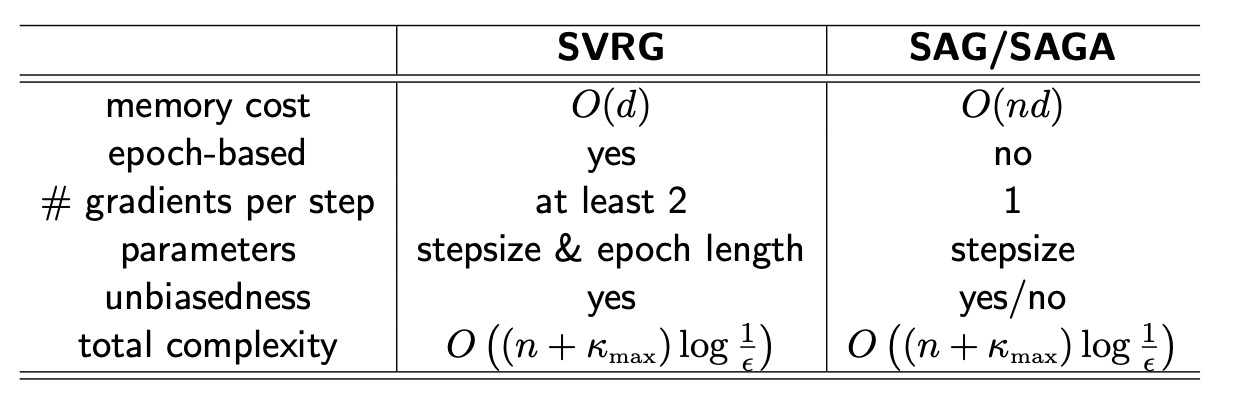
\includegraphics[width=\linewidth]{imgs/SVRG.jpg}
\begin{enumerate}
    \item \textbf{Stochastic average gradient (SAG)}: use average of the past gradient as an estimate of the full gradient: $g_t = \frac{1}{n}\sum_{i=1}^n v_i^t$, where $v_i^t = \nabla f_{i_t}(x_t)$ for $i=i_t$ and $v_i^t=v_i^{t-1}$ otherwise. Equivalently, $g_t = g_{t-1} + \frac{1}{n}(\nabla f_{i_t}(x_t) - v_{i_t}^{t-1})$. This means SAG is as cheap as SGD. It has convergence rate linear in $\log{1/\epsilon}$ for strongly convex and smooth functions.
    \item \textbf{SAGA}: use $g_t = \nabla f_{i_t}(x_t) - v_{i_t}^{t-1} + \frac{1}{n}\sum_{i=1}^n v_i^{t-1}$ to make it unbiased. It has the same rate as SAG.
    \item \textbf{Stochastic variance-reduced gradient (SVRG)}: use a fixed reference point to estimate the gradient: $g_t = \nabla f_{i_t}(x_{t}) - \nabla f_{i_t}(\tilde{x}) + \nabla F(\tilde{x})$ and $x_{t+1} = x_{t} - \eta g_t$, where the reference point $\tilde{x}_t$ is updated only once a while. Idea: $\E(\|g_t - \nabla F(x_t)\|^2) \le \E(\|\nabla f_{i_t}(x_t) - \nabla f_{i_t}(\tilde{x})\|^2) \le L_{\text{max}}^2\|x_t - \tilde{x}\|^2$, so the variance is bounded by how close $x_t$ is to $\tilde{x}$. Typical choice of $\tilde{x}$: each epoch $s$ consists of $m$ update, then use $\tilde{x}^s = \frac{1}{m}\sum_i x_t$ as the reference point of next epoch.
\end{enumerate}

\textbf{Convergence of SVRG}: (12.11) assume $f_i(x)$ is convex and $L$-smooth and $F(x)=\frac{1}{n}\sum_{i=1}^n f_i(x)$ is $\mu$-strongly convex. Let $x^*=\argmin_x F(x)$. For large $m$ and $\eta < \frac{1}{2L}$, and $\rho:=\frac{1}{\mu\eta(1-2L\eta)m}+\frac{2L\eta}{1-2L\eta} < 1$, we have $\E(F(\tilde{x}^s) - F(x^*)) \le \rho^s(F(\tilde{x}^0) - F(x^*))$. Proof: by $\|a+b\|^2\le 2\|a\|^2+2\|b\|^2$, we have $\E(\|g_t\|^2) \le 2\E(\|\nabla f_{i_t}(x_{t}) - \nabla f_{i_t}(x^*)\|^2) + 2\E(\|\nabla f_{i_t}(\tilde{x}) - \nabla f_{i_t}(x^*) - \nabla F(\tilde{x}^*)\|^2)$. Notice $\E(\|\nabla f_{i_t}(\tilde{x}) - \nabla f_{i_t}(x^*) - \nabla F(\tilde{x}^*)\|^2) = \E(\|\nabla f_{i_t}(\tilde{x}) - \nabla f_{i_t}(x^*)\|^2)$ and use lemma 12.12, we have $\E(\|g_t\|^2) \le 4L(F(x_{t}) - F(x^*) + F(\tilde{x}) - F(x^*))$. Therefore, $\E(\|x_{t+1}-x^*\|^2) = \|x_t - x^*\|^2 - 2\eta(x_t - x^*)^\top \E(g_t) + \eta^2\E(\|g_t\|^2) \le \|x_t - x^*\|^2 -2\eta(1-2L\eta)(F(x_t) - F(x^*)) + 4L\eta^2(F(\tilde{x}) - F(x^*))$. By convexity, we have $-\sum_{i=1}^m \E(F(x_{t} - F(x^*))) \le -m \E(F(\tilde{x}) - F(x^*))$. In addition, by strong convexity, we have $\E(\|\tilde{x} - x^*\|^2) \le \frac{2}{\mu}\E(F(\tilde{x}) - F(x^*))$. Combining these three gives the desired result. Set $\eta=O(1/L)$ and $m=O(L/\mu)$ makes $\rho \in (0, 0.5)$. Thus, the convergence is linear in $O(\log(1/\epsilon))$.

Other methods: 

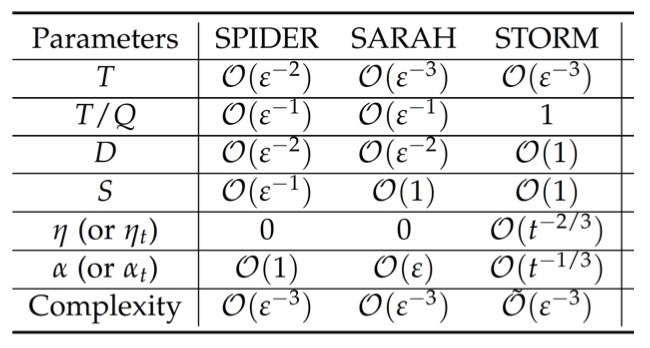
\includegraphics[width=\linewidth]{imgs/SGD-var.jpg}

\section{Nonconvex Functions}

\textbf{Smooth functions (no longer convex)}: $f$ is called $L$-smooth if $f(y) \le f(x)+\nabla f(x)^\top (y-x) + \frac{L}{2}\|y-x\|^2$. (9.1) If $\|\nabla^2 f(x)\|\le L$ for any $x$, then $f$ is smooth. For convex $f$ and \emph{open} $\dom(f)$, the reverse is also true.

\textbf{Gradient Descent for smooth functions}: (9.2) let $f$ has a global minimum $x^*$ and is $L$-smooth. With $\gamma=1/L$, GD yields $\frac{1}{T}\sum_t \|\nabla f(x_t)\|^2 \le \frac{2L}{T}(f(x_0) - f(x^*))$. Proof: by sufficient decrease, we have $\|\nabla f(x_t)\|^2 \le 2L(f(x_t) - f(x_{t+1}))$. Sum together gives the result.

\textbf{GD with $\gamma=1/L$ cannot overshoot}: (9.3) if $x$ is not a critical point, and $f$ is $L$-smooth over the line connecting $x$ and $x^\prime = x - \gamma \nabla f(x)$. Then with $\gamma = 1/L^\prime < 1/L$, $x^\prime$ is not a critical point. This means there is no critical point between $x$ and $x^\prime$, so no overshooting.

\textbf{Deciding whether a critical point is a local minimum is coNP-complete.}

\section{Frank-Wolfe Algorithm}

This is to solve constrained optimization, similar to PGD.

\textbf{Definitions}:
\begin{enumerate}
    \item \textbf{Linear minimization oracle (LMO)}: $\LMO_X(g) = \argmin_{z\in X} g^\top z$.
    \item \textbf{Frank-Wolfe algorithm}: do $s = \LMO_X(\nabla f(x_t))$ and $x_{t+1} = (1-\gamma_t)x_t+\gamma_t s$. Benefits: (1) the iterates are always feasible for convex domain; (2) the algorithm is projection-free if we can solve LMO; (3) the iterates have a sparse representation, defined by the combination of LMO in the previous steps; (4) it is affine-invariant, meaning that affine equivalent problems can be solved at the same cost, i.e., if $g(x)=f(Ax+b)$ and $\dom(g)=A^{-1}(\dom(f)-b)$, then minimizing $g$ is the same to minimizing $f$.
    \item \textbf{Curvature constant}: the curvature constant of the constrained optimization is defined to be $C_{f,X} = \sup_{y=(1-\gamma)x+\gamma s, \gamma \in (0,1]} \frac{1}{\gamma^2} (f(y) - f(x) - \nabla f(x)^\top (y-x))$. 
\end{enumerate}

\textbf{LASSO ($L_1$ domain)}: minimize $\|Ax-b\|^2$ subject to $\|x\|_1\le 1$. Thus, $\LMO_X(g) = \argmin_{z = \pm e_i, i\in [n]} g^\top z = -\sgn(g_i) e_i$, where $i = \argmax |g_i|$. Therefore, we can compute LMO in $O(\log(d))$.

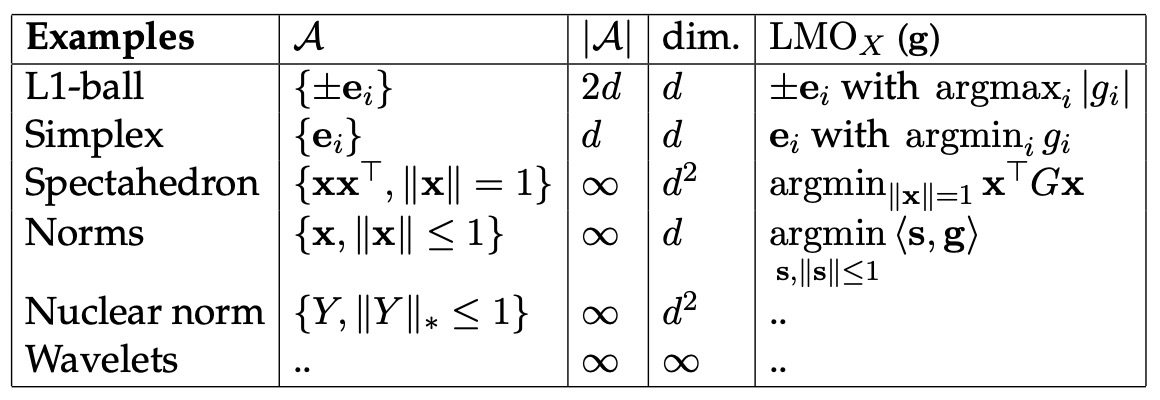
\includegraphics[width=\linewidth]{imgs/LMO.jpg}

\textbf{Duality gap as a certificate for optimization quality}: We define the duality gap at $x$ to be $g(x) = \nabla f(x)^\top (x-s)$, where $s = \LMO_X(\nabla f(x))$. (8.2) For convex $f$, $g(x) \ge f(x) - f(x^*)$. Proof: $g(x) = \nabla f(x)^\top x - \min_{z \in X} \nabla f(x)^\top z \ge \nabla f(x)^\top x - \nabla f(x)^\top x^* \ge f(x) - f(x^*)$.

\textbf{Analysis}:
\begin{enumerate}
    \item \textbf{Decrease property}: (8.4) for $\gamma_t \in [0,1]$, we have $f(x_{t+1}) \le f(x_t) - \gamma_t g(x_t) + \gamma_t^2 \frac{L}{2}\|s-x_t\|^2$, where $g(x_t)$ is the duality gap. Proof: by smoothness, $f(x_{t+1}) \le f(x_t) + \nabla f(x_t)^\top \gamma_t(s-x_t) + \gamma_t^2 \frac{L}{2}\|s-x_t\|^2 = f(x_t) - \gamma_t g(x_t) + \gamma_t^2 \frac{L}{2}\|s-x_t\|^2$.
    \item \textbf{Affine-invariant decrease}: we have $f(x_{t+1}) \le f(x_t) - \gamma_t g(x_t) + \gamma_t^2 C_{f,X}$. Proof: plug in $x=x_t$, $y=(1-\gamma_t)x_t+\gamma_t s$ into the definition of curvature constant.
    \item $\gamma_t = \frac{2}{t+2}$: (8.3) assume $f$ is convex and $L$-smooth, and $X$ is convex, closed and bounded, then $f(x_T) - f(x^*) \le \frac{2LR^2}{T+1}$, where $R = \max_{x,y\in X}\|x-y\|$. Proof: define $h(x) = f(x) - f(x^*)$, thus $h(x_{t+1}) \le h(x_t) - \gamma_t h(x_t) + \gamma_t^2 \frac{L}{2}\|s-x_t\|^2 \le (1-\gamma_t)h(x_t) + \gamma_t^2 C$, where $C = \frac{L}{2}R^2$. By induction, we have $h(x_t) \le \frac{4C}{t+1}$. (8.5) The same holds for $C_{f,X}$ instead of $C$.
    \item $\gamma_t^\prime = \argmin_{\gamma \in [0,1]} f((1-\gamma)x_t + \gamma s)$: the same result holds as now we have $h(x_{t+1}) \le h((1-\gamma_t)x_t + \gamma_t s) \le (1-\gamma_t)h(x_t) + \gamma_t^2 C$.
    \item $\gamma_t^\prime = \min(\frac{g(x_t)}{L\|s-x_t\|^2}, 1)$: the same result holds as now we have $h(x_{t+1}) \le h(x_t) - \gamma_t g(x_t) + \gamma_t^2 C$ as well, since $\gamma_t^\prime$ minimizes this upper bound.
    \item \textbf{Convergence of duality gap}: (8.7) under the same setting, $g(x_t) \le O(\frac{C_{f,X}}{T+1})$.
\end{enumerate}

\section{Newton's Method}

\textbf{Find zeros}: $x_{t+1} = x_t - \frac{f(x_t)}{f^\prime(x_t)}$. This is to solve the first-order approximation: $f(x_t)+f^\prime(x_t)(x-x_t) = 0$.

\textbf{Find minimum}: $x_{t+1} = x_t - \frac{f^\prime(x_t)}{f^{\prime\prime}(x_t)}$. This is to search zeros of $f^\prime$. Generally, $x_{t+1} = x_t - \nabla^2 f(x_t)^{-1} \nabla f(x_t)$. (10.3) $x_{t+1} = \argmin f(x_t) + \nabla f(x_t)^\top (x-x_t) + \frac{1}{2}(x-x_t)^\top \nabla^2 f(x_t) (x-x_t)$.

\textbf{Analysis}:
\begin{enumerate}
    \item \textbf{Nondegenerate quadratic function}: (10.1) for $f(x) = \frac{1}{2}x^\top M x - q^\top x +c$ with invertible symmetric $M$, Newton's method yields $x_1 = x^* = M^{-1} q$ for any $x_0$.
    \item \textbf{Affine invariance}: (10.2) let $f$ be twice differentiable, $A$ invertible and $g(y)=Ay+b$. Define $N_h(x) = x - \nabla^2 h(x)^{-1}\nabla h(x)$, then $N_{f\circ g}=g^{-1} \circ N_f \circ g$.
    \begin{center}
        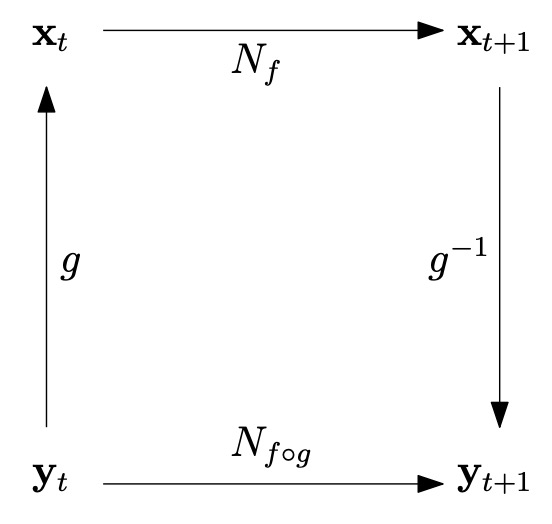
\includegraphics[width=.4\linewidth]{imgs/newton-affine.jpg}
    \end{center}
    \item \textbf{Bounded inverse Hessian and Lipschitz continuous Hessian}: (10.4) assume $f$ is twice continuously differentiable, $\|\nabla^2 f(x)^{-1}\| \le 1/\mu$ and $\|\nabla^{2} f(x) - \nabla^2 f(y)\| \le B\|x-y\|$ for any $x, y \in X$. Then we have $\|x_{t+1}-x^*\| \le \frac{B}{2\mu}\|x_t - x^*\|^2$ if a critical point $x^*$ exists in $X$. Proof: Define $H(x)=\nabla^2 f(x)$. $x_{t+1}-x^* = x_t - x^* + H(x_t)^{-1}(\nabla f(x^*) - \nabla f(x_t)) = x_t - x^* + H(x_t)^{-1} \int_0^1 H(x_t+u(x^*-x_t))(x^* - x_t) du = H(x_t)^{-1} \int_0^1 (H(x_t + u(x^* - x_t)) - H(x_t))(x^* - x_t) du$. Therefore, we have $\|x_{t+1}-x^*\| \le \|H(x_t)^{-1}\| \|x^* - x_t\| \int_0^1 \|H(x_t + u(x^* - x_t)) - H(x_t)\| du \le \frac{1}{\mu} \|x_t - x^*\|^2 B \int_0^1 u du = \frac{B}{2\mu} \|x_t-x^*\|^2$.
    \item \textbf{Fast convergence if near}: (10.5) under the assumption of (10.4), if $\|x_0-x^*\| \le \mu/B$, then $\|x_T - x^*\| \le \frac{\mu}{B}(\frac{1}{2})^{2^T-1}$. Proof: induction on (10.4).
    \item \textbf{Global convergence for strongly convex and smooth functions}: with $\gamma=\mu/L$, (scaled) Newton's method $x_{t+1}=x_t - \gamma \nabla^2 f(x_t)^{-1} \nabla f(x_t)$ satisfies $f(x_t) - f^* \le (1-\frac{\mu^2}{L^2})^t (f(x_0) - f^*)$. Note that the constant is worse than GD. Proof: expand $f(x_{t+1}) - f(x_t)$ by smoothness, then use $\frac{1}{L}\le \|H_t^{-1}\| \le \frac{1}{\mu}$ and $\|\nabla f(x_t)\|^2 \ge 2\mu (f(x_t)-f^*)$.
\end{enumerate}

\section{Quasi-Newton Methods}

Computing and inverting the Hessian in Newton's method is costly. Quasi-Newton methods want to avoid this.

\textbf{Secant condition}: use approximation $f^\prime(x_t) \approx \frac{f(x_t) - f(x_{t-1})}{x_t - x_{t-1}}$ to find zeros. Thus, the second method updates as: $x_{t+1} = x_t - f^\prime(x_t) \frac{x_t - x_{t-1}}{f^\prime(x_t) - f^\prime(x_{t-1})}$. To generalize to higher dimensions, we want to find $H_t$ such that $\nabla f(x_t) - \nabla f(x_{t-1}) = H_t(x_t - x_{t-1})$, and do $x_{t+1} = x_t - H_t^{-1} \nabla f(x_t)$.

\textbf{Quasi-Newton method}: if the method satisfies secant condition, we say it is a quasi-Newton method. In the multidimensional case, $H_t$ is not unique. In particular, Newton's method is a quasi-Newton method iff $f$ is a non-degenerate quadratic function. For efficiency, quasi-Newton methods typically deal with the inverse directly.

\textbf{Greenstadt's approach}: update $H_t^{-1} = H_{t-1}^{-1} + E_t$ for some symmetric $E_t$ with small $\|E_t\|_F^2 = \sum_{i,j} e_{i,j}^2$. To introduce more flexibility, we minimize $\|AE_t A^\top\|_F^2$ for some fixed invertible matrix $A$. The program is: minimize $\frac{1}{2}\|AE_t A^\top\|_F^2$ such that $E_t^\top = E_t$ and $E_t (\nabla f(x_t) - \nabla f(x_{t-1})) = x_t - x_{t-1} - H_{t-1}^{-1} (\nabla f(x_t) - \nabla f(x_{t-1}))$, which is the secant condition. Note that this is a convex program, so we solve by Lagrange method.

For simplicity, we write the program as: minimize $\frac{1}{2}\|AE A^\top\|_F^2$ such that $Ey=r$ and $E^\top - E=0$. Define $f(E) = \frac{1}{2}\|AE A^\top\|_F^2$, thus $\nabla f(E) = A^\top A E A^\top A$. Note that the constraints are in fact linear over $e_{i,j}$. (11.3) Define $M = (A^\top A)^{-1}$ which is positive definite, then a solution $E^*$ is optimal iff $E^*  = M(\lambda y^\top + \Gamma^\top - \Gamma)M$, where $\lambda \in \mathbb{R}^{d\times 1}$ and $\Gamma \in \mathbb{R}^{d\times d}$. Solving the linear system gives $E^* = \frac{1}{y^\top M y}(r y^\top M + M y r^\top - \frac{y^\top r}{y^\top M y} Myy^\top M)$. This is called the Greenstadt method with parameter $M$.

\textbf{BFGS}: BFGS (named after four people) is the Greenstadt method with parameter $H_t^{-1}$. Note that $H_t^{-1}$ is not yet known in the computation of $E_t$, but we have $H_t^{-1} y = x_t - x_{t-1}$ and in the formula of $E^*$, $M$ appears in the form of $My$. This allows us to compute $E^*$ without knowing the value of $M$. BFGS ensures that if $f$ is not flat between $x_{t-1}$ and $x_t$, and $H_{t-1}$ is positive definite, then $H_{t}$ is also positive definite. This reduces per iteration cost to $O(d^2)$.

\textbf{L-BFGS}: Define $\sigma = x_t - x_{t-1}$, $y = \nabla f(x_t) - \nabla f(x_{t-1})$, $H = H_{t-1}^{-1}$ and $H^\prime = H_t^{-1}$, then BFGS can be written as $ H^\prime = (I-\frac{\sigma y^\top}{y^\top \sigma}) H (I-\frac{ y \sigma^\top}{y^\top \sigma}) + \frac{\sigma \sigma^\top}{y^\top \sigma}$. L-BFGS relies on the efficient computation of $H^\prime g^\prime$ given that $H g$ can be computed efficiently for any $g$ and $g^\prime$. This is because $H^\prime g^\prime = (I-\frac{\sigma y^\top}{y^\top \sigma}) \left[H (I-\frac{ y \sigma^\top}{y^\top \sigma}) g^\prime\right] + \sigma \frac{\sigma^\top g^\prime}{y^\top \sigma}$ and note $(I-\frac{\sigma y^\top}{y^\top \sigma}) s = s - \sigma \frac{y^\top s}{y^\top \sigma}$, thus can be computed in $O(d)$ with one call of $Hg$. Recursively, we get $O(td)$ time complexity, which is not helpful. Instead, L-BFGS only does recursion for $m$ times, and use $H_0$ instead of $H_{t-m}$ (which is unknown to us as we do not explicitly compute this) as the result of $m$-th recursion. Note that we start close, so $H_0$ is close to $H_{t-m}$. In practice, we use a better choice than $H_0$.  The final complexity is $O(md)$ per iteration.

\section{Modern Second-order methods and nonconvex optimization}

\subsection{Cubic Regularization}

Motivation: for $L$-Lipschitz Hessian as in the assumption of Newton's method, we have $f(x) \le f(x_t) + \nabla f(x_t)^\top (x-x_t) + \frac{1}{2}(x-x_t)^\top \nabla^2 f(x_t) (x- x_t) + \frac{L}{6}\|x-x_t\|^3$. Similar to GD which minimizes the upper bound given by smoothness (Lipschitz gradient), cubic regularization is to minimize the upper bound given by Lipschitz Hessian. Algorithm: $x_{t+1} = \argmin_x f(x_t) + \nabla f(x_t)^\top (x-x_t) + \frac{1}{2}(x-x_t)^\top \nabla^2 f(x_t) (x- x_t) + \frac{L}{6}\|x-x_t\|^3$. This can be reduced to a convex problem.

\textbf{Convergence rate}: $\min_{i\le t} \|\nabla f(x_i)\| = O(t^{-2/3})$. If convex, we have $f(x_t) - f^* = O(t^{-2})$.

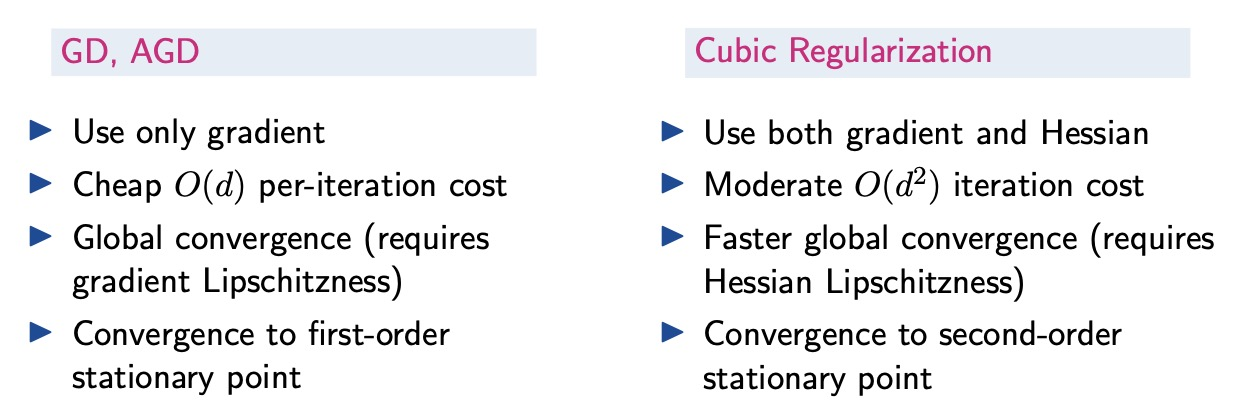
\includegraphics[width=\linewidth]{imgs/cubic.jpg}

\subsection{Nonconvex Optimization}

A nonconvex optimization may have exponentially many local minima, and determining whether a critical point is a local minimum is co-NP complete.

\textbf{Classification of stationary points}: (1) If $\nabla^2 F(x) \succ 0$, then $x$ is a local minimum; (2) If $\nabla^2 F(x) \prec 0$, then $x$ is a local maximum; (3) If $\nabla^2 F(x)$ has both positive and negative eigenvalues, then $x$ is a (strict) saddle point; (4) Otherwise, it remains inconclusive.

\textbf{Analysis}:
\begin{enumerate}
    \item \textbf{SGD converges to a stationary point}: see (12.8).
    \item \textbf{SGD with random initialization}: with random initialization, GD converges to a local minimum almost surely.
    \item \textbf{Noisy SGD}: with extra noise added to the SGD update, if $f$ satisfies strict saddle property and has Lipschitz Hessian, then noisy SGD converges to a second-order stationary point.
    \item \textbf{Benign landscapes}: if the function satisfies PL condition, or all local minimum is global minimum, then GD (in the latter case requires random initialization) converges to the global minimum.
\end{enumerate}

\section{Smoothing Techniques}


\subsection{Convex Conjugate}
\textbf{Convex conjugate (Legendre-Fenchel)}: for any $f$, its convex conjugate is given as $f^*(y) = \sup_{x\in \dom(f)} \{x^\top y - f(x)\}$.

\textbf{Properties}:
\begin{enumerate}
    \item \textbf{Fenchel's inequality}: $f(x)+f^*(y) \ge x^\top y$ for any $x, y$. Proof by definition.
    \item \textbf{Conjugate of a conjugate}: (7.2) If $f$ is convex, lower semi-continuous and proper, then $(f^*)^* = f$. A proper convex function means $f(x)>-\infty$.
    \item \textbf{Strong convexity implies nice conjugate}: (7.3) If $f$ is $\mu$-strongly convex, then $f^*$ is continuously differentiable and $\frac{1}{\mu}$ smooth.
    \item \textbf{Conjugate of function sum}: If $f$ and $g$ is lower semi-continuous and convex, then $(f+g)^*(x) = \inf_y\{f^*(y)+g^*(x-y)\}$.
\end{enumerate}

\subsection{Nesterov's Smoothing}
Use $f_\mu(x) = \max_{y \in \dom(f^*)} \{x^\top y - f^*(y) - \mu d(y)\}$ as the surrogate function to minimize. $d(y)$ is a $1$-strongly convex and nonnegative everywhere function, called the proximity function. Typical choices include $d(y) = \frac{1}{2}\|y-y_0\|^2$ and $d(y) = \frac{1}{2}\sum w_i(y_i - y_{0,i})^2$ for $w_i\ge 1$. This makes $f_\mu(x)$ to be $\frac{1}{\mu}$-smooth, as $f^*(y)+\mu d(y)$ is $\mu$-strongly convex.

\textbf{Approximation Error}: for convex $f$ with bounded $\dom(f^*)$, we have $f(x)-\mu D^2 \le f_\mu(x) \le f(x)$, where $D^2 = \max_{y\in\dom(f^*)} d(y)$. The tradeoff between approximation error and optimization error: $f(x) - f^* \le [f(x) - f_\mu(x)] + [f_\mu(x) - \min_x f_\mu(x)]$. With AGD, we get $f(x_t)- f^* = O(\mu D^2 + \frac{R^2}{\mu t^2})$. To achieve approximation error $\epsilon$, we need $\mu = O(\frac{\epsilon}{D^2})$. Therefore, $T_\epsilon = O(\frac{RD}{\epsilon})$.

\subsection{Moreau-Yosida Smoothing}

Use $f_{\mu}(x) = \min_y \{f(y) + \frac{1}{2\mu}\|x-y\|^2\}$. This is actually the special case of Nesterov's smoothing with $d(y)=\frac{1}{2}\|y\|^2$. Proof: $f_\mu^{Nes}(x) = \max_y\{x^\top y - f^*(y) - \frac{\mu}{2}\|y\|^2\}= (f^* + \frac{\mu}{2}\|\cdot\|^2)^*(x) = \inf_y \{f(y) + \frac{1}{2\mu}\|x-y\|^2\}$.

\textbf{Properties}: (1) $f_\mu(x)$ is $\frac{1}{\mu}$-smooth; (2) $\min_x f(x) = \min_x f_\mu(x)$. (3) GD reduces to proximal minimization: define $\prox_{\mu\cdot f} = \argmin_y \{f(y) + \frac{1}{2\mu}\|x-y\|^2\}$, then $x_{t+1} = x_t - \mu \nabla f_\mu(x_t) \Leftrightarrow x_{t+1} = \prox_{\mu\cdot f}(x_t)$.

\textbf{Proximal operator}: the proximal operator of convex function $f$ at $x$ is defined as $\prox_f(x) = \argmin_y\{f(y)+\frac{1}{2}\|x-y\|^2\}$. For continuous convex function $f$, $\prox_f(x)$ exists and is unique.

\textbf{Properties}:
\begin{enumerate}
    \item \textbf{Fixed point}: If $f$ is convex, then $x^* \in \argmin f(x) \Leftrightarrow x^* = \prox_f(x^*)$. Proof by definition.
    \item \textbf{Non-expansive}: $\|\prox_f(x) - \prox_f(y)\| \le \|x-y\|$. Proof: Let $\mu_x = \prox_f(x)$ and $\mu_y = \prox_f(y)$. By optimality condition, $x - \mu_x \in \partial f(\mu_x)$ and $y - \mu_y \in \partial f(\mu_y)$. By the monotonicity of gradient, $(x-\mu_x - (y-\mu_y))^\top (\mu_x - \mu_y) \ge 0$. This means $\|\mu_x - \mu_y\|^2 \le (x-y)^\top (\mu_x - \mu_y) \le \|x-y\|\|\mu_x - \mu_y\|$.
    \item \textbf{Moreau decomposition}: For any $x$, $x = \prox_f(x) + \prox_{f^*}(x)$. Proof: use $u_x \in \partial f^*(x-u_x)$.
\end{enumerate}

\textbf{Proximal Point Algorithm}: $x_{t+1} = \prox_{\gamma_t\cdot f}(x_t)$. (7.14) If $f$ is convex, then $f(x_{T}) - f^* \le \frac{\|x_0 - x^*\|^2}{2\sum_{t=0}^{T-1} \gamma_t}$. Proof: by definition, $f(x_{t+1}) + \frac{1}{2\gamma_t} \|x_{t+1} - x_t\|^2 \le f(x_t)$, which implies $f(x_{t+1}) - f(x_t) \le -\frac{1}{2\gamma_t} \|x_{t+1}-x_t\|^2$. By optimality condition, $0 \in \partial f(x_{t+1}) + \frac{1}{\gamma_t}(x_{t+1} - x_t)$, which implies $\frac{x_t - x_{t+1}}{\gamma_t} \in \partial f(x_{t+1})$. Therefore, by the definition of subgradient, $f(x_{t+1}) - f^* \le \frac{1}{\gamma_t} (x_t - x_{t+1})^\top (x_{t+1} - x^*) \le \frac{1}{\gamma_t} [(x_t - x^*)^\top (x_{t+1} - x^*) - \|x_{t+1} - x^*\|^2]$. Using $(x_t - x^*)^\top (x_{t+1} - x^*) \le \frac{1}{2}(\|x_t - x^*\|^2 + \|x_{t+1} - x^*\|^2)$, we get $ f(x_{t+1}) - f^* \le \frac{1}{2\gamma_t}[\|x_t - x^*\|^2 - \|x_{t+1} - x^*\|^2]$. The rest follows from non-increasing $f(x_t)$ and summing this inequality by $t$.

\subsection{Lasry-Lions Smoothing}

Use $f_{\mu,\delta}(x) = \max_y \min_z \{f(z) + \frac{1}{2\mu}\|z-y\|^2 - \frac{1}{2\delta} \|y-x\|^2\}$. This is double application of Moreau smoothing with function flipping. If $f$ is 1-Lipschitz, then choose $\delta,\mu = O(\epsilon)$ guarantees $\epsilon$ approximation error, and $f_{\mu,\delta}$ is $O(1/\epsilon)$-smooth. This can be applied to nonconvex functions, but has computation inefficiency in this case. 

\subsection{Randomized Smoothing}

Use $f_\mu(x) = \E_z[f(x + \mu z)]$, where $z$ is an isotopic Gaussian or uniform random variable. Choosing $\mu = O(\epsilon)$ guarantees $\epsilon$ approximation error, and $f_\mu(x)$ is $O(\frac{\sqrt{d}}{\epsilon})$-smooth.

\section{Min-Max Optimization}

The min-max problem is defined as $\min_{x\in X} \max_{y \in Y} \phi(x,y)$.

\textbf{Definitions}:
\begin{enumerate}
    \item \textbf{Saddle point and minimax point}: $(x^*, y^*)$ is a saddle point if $\phi(x^*, y) \le \phi(x^*, y^*) \le \phi(x, y^*)$ for any $x, y$. $(x^*, y^*)$ is a global minimax point if $\phi(x^*, y) \le \phi(x^*, y^*) \le \max_{y^\prime \in Y} \phi(x, y^\prime)$ for any $x, y$. Game theory interpretation: saddle point means Nash equilibrium, where no play has the incentive to make unilateral changes; global minimax point is Stackelberg equilibrium, where it is the best response to the best response.
    \item \textbf{Convex-concave function}: $\phi(x, y)$ is convex-concave if $\phi(x, y)$ is convex for every fixed $y$ and $\phi(x,y)$ is concave for every fixed $x$.
    \item \textbf{Strongly-convex-strongly-concave function}: $\phi(x, y)$ is strongly-convex-strongly-concave if $\phi(x, y)$ is $\mu_1$-strongly convex for every fixed $y$ and $\phi(x,y)$ is $\mu_2$-strongly concave for every fixed $x$.
    \item \textbf{Smoothness jointly in $x$ and $y$}: $\|\nabla_x \phi(x_1, y_1) - \nabla_x \phi(x_2, y_2)\| \le L(\|x_1 - x_2\| + \|y_1 - y_2\|)$ and $\|\nabla_y \phi(x_1, y_1) - \nabla_y \phi(x_2, y_2)\| \le L(\|x_1 - x_2\| + \|y_1 - y_2\|)$.
    \item \textbf{Duality gap}: defined to be $\max_y \phi(\hat{x}, y) - \min_x \phi(x, \hat{y})$. When duality gap is smaller than or equal to $\epsilon$, we say $(\hat{x}, \hat{y})$ is an $\epsilon$-saddle point.
    \item \textbf{Monotone operators}: A operator $F$ is monotone if $(F(u) - F(v))^\top (u-v) \ge 0$ for any $u,v$; it is $\mu$-strongly monotone if $(F(u) - F(v))^\top (u-v) \ge \mu \|u-v\|^2$ for any $u,v$.
\end{enumerate}

\textbf{Properties}:
\begin{enumerate}
    \item \textbf{Characterization of saddle points}: Define $\bar{\phi}(x) = \max_y \phi(x,y)$ and $\underline{\phi}(y) = \min_x \phi(x,y)$. Then $(x^*, y^*)$ is a saddle point iff $\max_y \min_x \phi(x,y) = \min_x \max_y \phi(x,y)$, $x^* \in \argmin_x \bar{\phi(x)}$ and $y^* \in \argmax_y \underline{\phi}(y)$. Proof: by definition.
    \item \textbf{Minimax Theorem}: If $X$ and $Y$ are closed convex sets, one of them is bounded, and $\phi(x,y)$ is a continuous convex-concave function, then there exists a saddle point on $X \times Y$ and $\max_y \min_x \phi(x, y) = \min \max \phi(x, y)$.
\end{enumerate}

\textbf{Gradient Descent Ascent}: do $x_{t+1} = \Pi_X(x_t - \gamma \nabla_x \phi(x_t, y_t))$ and $y_{t+1} = \Pi_Y (y_t + \gamma \nabla_y \phi(x_t, y_t))$. This simultaneously updates $x$ and $y$.

\textbf{Analysis}:
\begin{enumerate}
    \item \textbf{SC-SC and smooth fucntions}: (12.5) with $\gamma = \frac{\mu}{4L^2}$, GDA converges linearly: $\|x_{t+1} - x^*\|^2 + \|y_{t+1} - y^*\|^2 \le (1-4\mu^2/L^2)(\|x_t - x^*\|^2 + \|y_t - y^*\|^2)$. Proof: by SC-SC, $(\nabla_x f(x,y) - \nabla_x f(x^*, y^*))^\top (x - x^*) + (\nabla_y f(x^*, y^*) - \nabla_y f(x,y))^\top (y-y^*) \ge \mu\|x - x^*\|^2 + \mu\|y-y^*\|^2$. By smoothness, $\|\nabla_x \phi(x_1, y_1) - \nabla_x \phi(x_2, y_2)\|^2 + \|\nabla_y \phi(x_1, y_1) - \nabla_y \phi(x_2, y_2)\|^2 \le 4L(\|x_1 - x_2\|^2 + \|y_1 - y_2\|^2)$. Using these in the update gives the result.
    \item \textbf{C-C functions}: may not converge, e.g. $\phi(x,y) = xy$. Proof: $x_{t+1}^2 + y_{t+1}^2 = (x_t - \gamma y_t)^2 + (y_t + \gamma x_t)^2 = (1+\gamma^2)(x_t^2 + y_t^2)$.
\end{enumerate}

\textbf{Extragradient Method}: 

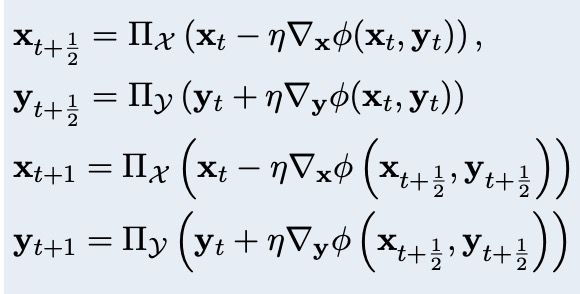
\includegraphics[width=\linewidth]{imgs/EG.jpg}

This is different from two steps of GDA, because the second step still uses the value of $t$. Essentially, EG is to use better gradients than GDA. EG has $O(1/T)$ convergece rate of the duality gap for averaged $x_{t+1/2}$ and $y_{t+1/2}$ in the C-C setting with bounded domain, and $O(\log(\frac{1}{\epsilon}))$ complexity in the SC-SC setting, which is optimal.

\textbf{Optimistic GDA}

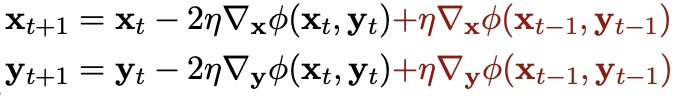
\includegraphics[width=\linewidth]{imgs/OGDA.jpg}

This is equivalent to:

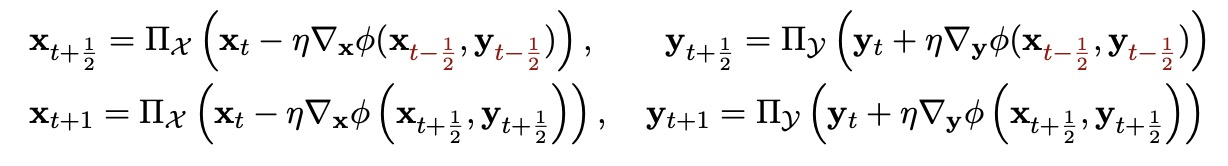
\includegraphics[width=\linewidth]{imgs/OGDA2.jpg}

OGDA has similar convergence rate as EG in the SC-SC and C-C settings.

\textbf{Proximal Point Algorithm}

do $(x_{t+1}, y_{t+1}) = \argmin_x \argmax_y \{\phi(x,y) + \frac{1}{2\eta} \|x-x_t\|^2 - \frac{1}{2\eta} \|y - y_t\|^2\}$.

This is equivalent to

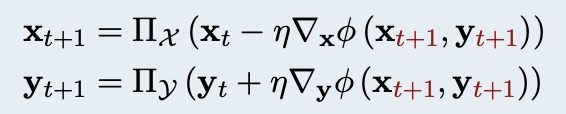
\includegraphics[width=\linewidth]{imgs/PPA.jpg}

PPA converges with $O(1/T)$ in the C-C setting. PPA, EG, OGDA and GDA are all using some estimation of the gradient.

\textbf{Concave games}: finite number of players $\mathcal{N} = \{1,\dots,N\}$, compact convex action set $X_i$, the utility function $u_i(x_i, x_{-i})$ is concave in $x_i$ for all $x_{-i}$.

\textbf{Nash equilibrium for concave games}: $u_i(x^*_i, x^*_{-i}) \ge u_i(x_i, x^*_{-i})$ for any $x_i \in X_i$. First-order characterization: in the concave game, Nash equilibria can be characterized as $\nabla_i u_i(x^*_i, x^*_{-i})^\top (x_i-x^*_i) \le 0$.

\textbf{Variational inequality problem}: find $z^* \in Z$ such that $F(z^*)^\top (z-z^*) \ge 0$ for all $z \in Z$. Existence: If $Z$ is a nonempty convex compact set and $F$ is continuous, then VI has a solution.

\textbf{Strong and weak solution of VI}: $z^*$ is a strong solution if $F(z^*)^\top (z-z^*) \ge 0$ for any $z$; $z^*$ is a weak solution if $F(z)^\top (z-z^*) \ge 0$. If $F$ is monotone, then a strong solution is a weak solution; If $F$ is continuous, then a weak solution is a strong solution.

\textbf{Min-max is a special case of VI}: let $F = (\nabla_x \phi, -\nabla_y \phi(y))$ makes it a VI. A point is a solution to this VI iff it is a saddle point.

\textbf{Solving VI by EG}: assume $Z$ is a closed convex set, the VI problem has solutions, $F$ is monotone and $L$-Lipschitz continuous, then EG: $\tilde{z_{t+1}} = \Pi_Z(z_t - \eta_t F(z_t))$ and $z_{t+1} = \Pi_Z(z_t - \eta_t F(\tilde(z)_{t+1}))$ converges in $O(1/T)$.

\end{multicols*}
\end{document}
